
%% bare_conf.tex
%% V1.3
%% 2007/01/11
%% by Michael Shell
%% See:
%% http://www.michaelshell.org/
%% for current contact information.
%%
%% This is a skeleton file demonstrating the use of IEEEtran.cls
%% (requires IEEEtran.cls version 1.7 or later) with an IEEE conference paper.
%%
%% Support sites:
%% http://www.michaelshell.org/tex/ieeetran/
%% http://www.ctan.org/tex-archive/macros/latex/contrib/IEEEtran/
%% and
%% http://www.ieee.org/

%%*************************************************************************
%% Legal Notice:
%% This code is offered as-is without any warranty either expressed or
%% implied; without even the implied warranty of MERCHANTABILITY or
%% FITNESS FOR A PARTICULAR PURPOSE! 
%% User assumes all risk.
%% In no event shall IEEE or any contributor to this code be liable for
%% any damages or losses, including, but not limited to, incidental,
%% consequential, or any other damages, resulting from the use or misuse
%% of any information contained here.
%%
%% All comments are the opinions of their respective authors and are not
%% necessarily endorsed by the IEEE.
%%
%% This work is distributed under the LaTeX Project Public License (LPPL)
%% ( http://www.latex-project.org/ ) version 1.3, and may be freely used,
%% distributed and modified. A copy of the LPPL, version 1.3, is included
%% in the base LaTeX documentation of all distributions of LaTeX released
%% 2003/12/01 or later.
%% Retain all contribution notices and credits.
%% ** Modified files should be clearly indicated as such, including  **
%% ** renaming them and changing author support contact information. **
%%
%% File list of work: IEEEtran.cls, IEEEtran_HOWTO.pdf, bare_adv.tex,
%%                    bare_conf.tex, bare_jrnl.tex, bare_jrnl_compsoc.tex
%%*************************************************************************

% *** Authors should verify (and, if needed, correct) their LaTeX system  ***
% *** with the testflow diagnostic prior to trusting their LaTeX platform ***
% *** with production work. IEEE's font choices can trigger bugs that do  ***
% *** not appear when using other class files.                            ***
% The testflow support page is at:
% http://www.michaelshell.org/tex/testflow/



% Note that the a4paper option is mainly intended so that authors in
% countries using A4 can easily print to A4 and see how their papers will
% look in print - the typesetting of the document will not typically be
% affected with changes in paper size (but the bottom and side margins will).
% Use the testflow package mentioned above to verify correct handling of
% both paper sizes by the user's LaTeX system.
%
% Also note that the "draftcls" or "draftclsnofoot", not "draft", option
% should be used if it is desired that the figures are to be displayed in
% draft mode.
%
\documentclass[conference]{IEEEtran}
% Add the compsoc option for Computer Society conferences.
%
% If IEEEtran.cls has not been installed into the LaTeX system files,
% manually specify the path to it like:
% \documentclass[conference]{../sty/IEEEtran}

\usepackage{pdfsync}
\usepackage{comment}
\usepackage{amsmath}
\usepackage{amssymb}
\usepackage{amsthm}
\usepackage{calc}
\usepackage{color}
\usepackage{graphicx}
\usepackage{url}
\usepackage{xspace}
\usepackage{tikz}
\usepackage{pgfplots}
\usepackage{caption}
\usepackage{subcaption}
\usepackage{xspace}

\usepackage[algo2e, noend, noline, linesnumbered]{algorithm2e}
\DontPrintSemicolon

\makeatletter
\newcommand{\pushline}{\Indp}% Indent
\newcommand{\popline}{\Indm}
\makeatother
\DeclareMathOperator{\pess}{pess}
\DeclareMathOperator{\opti}{opti}
\newcommand{\argmax}{\operatornamewithlimits{argmax}}

\captionsetup{compatibility=false}


%\usepackage{subfig}


% the note center!
%\newcommand{\marcl}[1]{\textbf{\color{red} #1 -- ML}}
%\newcommand{\rgg}[1]{\textbf{\color{red} #1 -- RG}}
\definecolor{darkgreen}{RGB}{0,125,0}
\newcounter{mwNoteCounter}
\newcounter{mlNoteCounter}
\newcounter{mtNoteCounter}
\newcommand{\mwinands}[1]{{\small \color{blue} $\blacksquare$ \refstepcounter{mwNoteCounter}\textsf{[RGG]$_{\arabic{mwNoteCounter}}$:{#1}}}}
\newcommand{\mlanctot}[1]{{\small \color{darkgreen} $\blacksquare$ \refstepcounter{mlNoteCounter}\textsf{[ML]$_{\arabic{mlNoteCounter}}$:{#1}}}}
\newcommand{\mtak}[1]{{\small \color{red} $\blacktriangle$ \refstepcounter{ntNoteCounter}\textsf{[MJ]$_{\arabic{mtNoteCounter}}$:{#1}}}}
%\newcounter{NoteCounter}
%\newcommand{\vlnote}[1]{{\scriptsize \color{blue} \refstepcounter{vlNoteCounter}\textsf{[VL]$_{\arabic{vlNoteCounter}}$:{#1}}}}
%\renewcommand{\vlnote}[1]{}

\newcommand{\bE}{\mathbb{E}}
\newcommand{\cA}{\mathcal{A}}
\newcommand{\cC}{\mathcal{C}}
\newcommand{\cD}{\mathcal{D}}
\newcommand{\cI}{\mathcal{I}}
\newcommand{\cN}{\mathcal{N}}
\newcommand{\cO}{\mathcal{O}}
\newcommand{\cS}{\mathcal{S}}
\newcommand{\cT}{\mathcal{T}}
\newcommand{\cZ}{\mathcal{Z}}
\newcommand{\eg}{{\it e.g.,}~}
\newcommand{\ie}{{\it i.e.,}~}
\newcommand{\Cadiaplayer}{{\sc CadiaPlayer}\xspace}


% Some very useful LaTeX packages include:
% (uncomment the ones you want to load)


% *** MISC UTILITY PACKAGES ***
%
%\usepackage{ifpdf}
% Heiko Oberdiek's ifpdf.sty is very useful if you need conditional
% compilation based on whether the output is pdf or dvi.
% usage:
% \ifpdf
%   % pdf code
% \else
%   % dvi code
% \fi
% The latest version of ifpdf.sty can be obtained from:
% http://www.ctan.org/tex-archive/macros/latex/contrib/oberdiek/
% Also, note that IEEEtran.cls V1.7 and later provides a builtin
% \ifCLASSINFOpdf conditional that works the same way.
% When switching from latex to pdflatex and vice-versa, the compiler may
% have to be run twice to clear warning/error messages.






% *** CITATION PACKAGES ***
%
%\usepackage{cite}
% cite.sty was written by Donald Arseneau
% V1.6 and later of IEEEtran pre-defines the format of the cite.sty package
% \cite{} output to follow that of IEEE. Loading the cite package will
% result in citation numbers being automatically sorted and properly
% "compressed/ranged". e.g., [1], [9], [2], [7], [5], [6] without using
% cite.sty will become [1], [2], [5]--[7], [9] using cite.sty. cite.sty's
% \cite will automatically add leading space, if needed. Use cite.sty's
% noadjust option (cite.sty V3.8 and later) if you want to turn this off.
% cite.sty is already installed on most LaTeX systems. Be sure and use
% version 4.0 (2003-05-27) and later if using hyperref.sty. cite.sty does
% not currently provide for hyperlinked citations.
% The latest version can be obtained at:
% http://www.ctan.org/tex-archive/macros/latex/contrib/cite/
% The documentation is contained in the cite.sty file itself.






% *** GRAPHICS RELATED PACKAGES ***
%
\ifCLASSINFOpdf
  % \usepackage[pdftex]{graphicx}
  % declare the path(s) where your graphic files are
  % \graphicspath{{../pdf/}{../jpeg/}}
  % and their extensions so you won't have to specify these with
  % every instance of \includegraphics
  % \DeclareGraphicsExtensions{.pdf,.jpeg,.png}
\else
  % or other class option (dvipsone, dvipdf, if not using dvips). graphicx
  % will default to the driver specified in the system graphics.cfg if no
  % driver is specified.
  % \usepackage[dvips]{graphicx}
  % declare the path(s) where your graphic files are
  % \graphicspath{{../eps/}}
  % and their extensions so you won't have to specify these with
  % every instance of \includegraphics
  % \DeclareGraphicsExtensions{.eps}
\fi
% graphicx was written by David Carlisle and Sebastian Rahtz. It is
% required if you want graphics, photos, etc. graphicx.sty is already
% installed on most LaTeX systems. The latest version and documentation can
% be obtained at: 
% http://www.ctan.org/tex-archive/macros/latex/required/graphics/
% Another good source of documentation is "Using Imported Graphics in
% LaTeX2e" by Keith Reckdahl which can be found as epslatex.ps or
% epslatex.pdf at: http://www.ctan.org/tex-archive/info/
%
% latex, and pdflatex in dvi mode, support graphics in encapsulated
% postscript (.eps) format. pdflatex in pdf mode supports graphics
% in .pdf, .jpeg, .png and .mps (metapost) formats. Users should ensure
% that all non-photo figures use a vector format (.eps, .pdf, .mps) and
% not a bitmapped formats (.jpeg, .png). IEEE frowns on bitmapped formats
% which can result in "jaggedy"/blurry rendering of lines and letters as
% well as large increases in file sizes.
%
% You can find documentation about the pdfTeX application at:
% http://www.tug.org/applications/pdftex





% *** MATH PACKAGES ***
%
%\usepackage[cmex10]{amsmath}
% A popular package from the American Mathematical Society that provides
% many useful and powerful commands for dealing with mathematics. If using
% it, be sure to load this package with the cmex10 option to ensure that
% only type 1 fonts will utilized at all point sizes. Without this option,
% it is possible that some math symbols, particularly those within
% footnotes, will be rendered in bitmap form which will result in a
% document that can not be IEEE Xplore compliant!
%
% Also, note that the amsmath package sets \interdisplaylinepenalty to 10000
% thus preventing page breaks from occurring within multiline equations. Use:
%\interdisplaylinepenalty=2500
% after loading amsmath to restore such page breaks as IEEEtran.cls normally
% does. amsmath.sty is already installed on most LaTeX systems. The latest
% version and documentation can be obtained at:
% http://www.ctan.org/tex-archive/macros/latex/required/amslatex/math/





% *** SPECIALIZED LIST PACKAGES ***
%
%\usepackage{algorithmic}
% algorithmic.sty was written by Peter Williams and Rogerio Brito.
% This package provides an algorithmic environment fo describing algorithms.
% You can use the algorithmic environment in-text or within a figure
% environment to provide for a floating algorithm. Do NOT use the algorithm
% floating environment provided by algorithm.sty (by the same authors) or
% algorithm2e.sty (by Christophe Fiorio) as IEEE does not use dedicated
% algorithm float types and packages that provide these will not provide
% correct IEEE style captions. The latest version and documentation of
% algorithmic.sty can be obtained at:
% http://www.ctan.org/tex-archive/macros/latex/contrib/algorithms/
% There is also a support site at:
% http://algorithms.berlios.de/index.html
% Also of interest may be the (relatively newer and more customizable)
% algorithmicx.sty package by Szasz Janos:
% http://www.ctan.org/tex-archive/macros/latex/contrib/algorithmicx/




% *** ALIGNMENT PACKAGES ***
%
%\usepackage{array}
% Frank Mittelbach's and David Carlisle's array.sty patches and improves
% the standard LaTeX2e array and tabular environments to provide better
% appearance and additional user controls. As the default LaTeX2e table
% generation code is lacking to the point of almost being broken with
% respect to the quality of the end results, all users are strongly
% advised to use an enhanced (at the very least that provided by array.sty)
% set of table tools. array.sty is already installed on most systems. The
% latest version and documentation can be obtained at:
% http://www.ctan.org/tex-archive/macros/latex/required/tools/


%\usepackage{mdwmath}
%\usepackage{mdwtab}
% Also highly recommended is Mark Wooding's extremely powerful MDW tools,
% especially mdwmath.sty and mdwtab.sty which are used to format equations
% and tables, respectively. The MDWtools set is already installed on most
% LaTeX systems. The lastest version and documentation is available at:
% http://www.ctan.org/tex-archive/macros/latex/contrib/mdwtools/


% IEEEtran contains the IEEEeqnarray family of commands that can be used to
% generate multiline equations as well as matrices, tables, etc., of high
% quality.


%\usepackage{eqparbox}
% Also of notable interest is Scott Pakin's eqparbox package for creating
% (automatically sized) equal width boxes - aka "natural width parboxes".
% Available at:
% http://www.ctan.org/tex-archive/macros/latex/contrib/eqparbox/





% *** SUBFIGURE PACKAGES ***
%\usepackage[tight,footnotesize]{subfigure}
% subfigure.sty was written by Steven Douglas Cochran. This package makes it
% easy to put subfigures in your figures. e.g., "Figure 1a and 1b". For IEEE
% work, it is a good idea to load it with the tight package option to reduce
% the amount of white space around the subfigures. subfigure.sty is already
% installed on most LaTeX systems. The latest version and documentation can
% be obtained at:
% http://www.ctan.org/tex-archive/obsolete/macros/latex/contrib/subfigure/
% subfigure.sty has been superceeded by subfig.sty.



%\usepackage[caption=false]{caption}
%\usepackage[font=footnotesize]{subfig}
% subfig.sty, also written by Steven Douglas Cochran, is the modern
% replacement for subfigure.sty. However, subfig.sty requires and
% automatically loads Axel Sommerfeldt's caption.sty which will override
% IEEEtran.cls handling of captions and this will result in nonIEEE style
% figure/table captions. To prevent this problem, be sure and preload
% caption.sty with its "caption=false" package option. This is will preserve
% IEEEtran.cls handing of captions. Version 1.3 (2005/06/28) and later 
% (recommended due to many improvements over 1.2) of subfig.sty supports
% the caption=false option directly:
%\usepackage[caption=false,font=footnotesize]{subfig}
%
% The latest version and documentation can be obtained at:
% http://www.ctan.org/tex-archive/macros/latex/contrib/subfig/
% The latest version and documentation of caption.sty can be obtained at:
% http://www.ctan.org/tex-archive/macros/latex/contrib/caption/




% *** FLOAT PACKAGES ***
%
%\usepackage{fixltx2e}
% fixltx2e, the successor to the earlier fix2col.sty, was written by
% Frank Mittelbach and David Carlisle. This package corrects a few problems
% in the LaTeX2e kernel, the most notable of which is that in current
% LaTeX2e releases, the ordering of single and double column floats is not
% guaranteed to be preserved. Thus, an unpatched LaTeX2e can allow a
% single column figure to be placed prior to an earlier double column
% figure. The latest version and documentation can be found at:
% http://www.ctan.org/tex-archive/macros/latex/base/



%\usepackage{stfloats}
% stfloats.sty was written by Sigitas Tolusis. This package gives LaTeX2e
% the ability to do double column floats at the bottom of the page as well
% as the top. (e.g., "\begin{figure*}[!b]" is not normally possible in
% LaTeX2e). It also provides a command:
%\fnbelowfloat
% to enable the placement of footnotes below bottom floats (the standard
% LaTeX2e kernel puts them above bottom floats). This is an invasive package
% which rewrites many portions of the LaTeX2e float routines. It may not work
% with other packages that modify the LaTeX2e float routines. The latest
% version and documentation can be obtained at:
% http://www.ctan.org/tex-archive/macros/latex/contrib/sttools/
% Documentation is contained in the stfloats.sty comments as well as in the
% presfull.pdf file. Do not use the stfloats baselinefloat ability as IEEE
% does not allow \baselineskip to stretch. Authors submitting work to the
% IEEE should note that IEEE rarely uses double column equations and
% that authors should try to avoid such use. Do not be tempted to use the
% cuted.sty or midfloat.sty packages (also by Sigitas Tolusis) as IEEE does
% not format its papers in such ways.





% *** PDF, URL AND HYPERLINK PACKAGES ***
%
%\usepackage{url}
% url.sty was written by Donald Arseneau. It provides better support for
% handling and breaking URLs. url.sty is already installed on most LaTeX
% systems. The latest version can be obtained at:
% http://www.ctan.org/tex-archive/macros/latex/contrib/misc/
% Read the url.sty source comments for usage information. Basically,
% \url{my_url_here}.





% *** Do not adjust lengths that control margins, column widths, etc. ***
% *** Do not use packages that alter fonts (such as pslatex).         ***
% There should be no need to do such things with IEEEtran.cls V1.6 and later.
% (Unless specifically asked to do so by the journal or conference you plan
% to submit to, of course. )


% correct bad hyphenation here
%\hyphenation{op-tical net-works semi-conduc-tor}


\begin{document}
%
% paper title
% can use linebreaks \\ within to get better formatting as desired
\title{Monte Carlo Tree Search Variants for\\Simultaneous Move Games}


% author names and affiliations
% use a multiple column layout for up to three different
% affiliations

%\author{Author1 Author2 Author3 Author4}

\author{\IEEEauthorblockN{Mandy J.~W. Tak, Marc Lanctot, and Mark H.~M.~Winands}
\IEEEauthorblockA{Department of Knowledge Engineering, Maastricht University\\
%P.O. Box 616, 6200 MD Maastricht, The Netherlands,\\
\{mandy.tak,marc.lanctot,m.winands\}@maastrichtuniversity.nl\\
}
}
%\IEEEauthorblockA{Twentieth Century Fox\\
%Springfield, USA\\
%Email: homer@thesimpsons.com}
%\and
%\IEEEauthorblockN{James Kirk\\ and Montgomery Scott}
%\IEEEauthorblockA{Starfleet Academy\\
%San Francisco, California 96678-2391\\
%Telephone: (800) 555--1212\\
%Fax: (888) 555--1212}}

% conference papers do not typically use \thanks and this command
% is locked out in conference mode. If really needed, such as for
% the acknowledgment of grants, issue a \IEEEoverridecommandlockouts
% after \documentclass

% for over three affiliations, or if they all won't fit within the width
% of the page, use this alternative format:
% 
%\author{\IEEEauthorblockN{Michael Shell\IEEEauthorrefmark{1},
%Homer Simpson\IEEEauthorrefmark{2},
%James Kirk\IEEEauthorrefmark{3}, 
%Montgomery Scott\IEEEauthorrefmark{3} and
%Eldon Tyrell\IEEEauthorrefmark{4}}
%\IEEEauthorblockA{\IEEEauthorrefmark{1}School of Electrical and Computer Engineering\\
%Georgia Institute of Technology,
%Atlanta, Georgia 30332--0250\\ Email: see http://www.michaelshell.org/contact.html}
%\IEEEauthorblockA{\IEEEauthorrefmark{2}Twentieth Century Fox, Springfield, USA\\
%Email: homer@thesimpsons.com}
%\IEEEauthorblockA{\IEEEauthorrefmark{3}Starfleet Academy, San Francisco, California 96678-2391\\
%Telephone: (800) 555--1212, Fax: (888) 555--1212}
%\IEEEauthorblockA{\IEEEauthorrefmark{4}Tyrell Inc., 123 Replicant Street, Los Angeles, California 90210--4321}}




% use for special paper notices
%\IEEEspecialpapernotice{(Invited Paper)}




% make the title area
\maketitle


\begin{abstract}
%\boldmath
Monte Carlo Tree Search (MCTS) is a widely-used technique for game-tree search in sequential turn-based games. 
The extension to simultaneous move games, where all player choose moves simultaneously each turn, 
is non-trivial due to the complexity of this class of games. In this paper, we describe simultaneous move MCTS 
and analyze its application in over a set of nine disparate simultaneous move games. We use several possible 
variants, Decoupled UCT, Sequential UCT, Exp3, and Regret Matching. These variants include both 
deterministic and stochastic selection strategies and we characterize the game-play performance of each one. 
The results indicate that the relative performance of 
each variant depends strongly on the game and the opponent, and that parameter tuning can also not be as 
straightforward as the purely sequential case. Overall, Decoupled UCT performs best in these games, despite its 
theoretical shortcomings. 
\end{abstract}
% IEEEtran.cls defaults to using nonbold math in the Abstract.
% This preserves the distinction between vectors and scalars. However,
% if the conference you are submitting to favors bold math in the abstract,
% then you can use LaTeX's standard command \boldmath at the very start
% of the abstract to achieve this. Many IEEE journals/conferences frown on
% math in the abstract anyway.

% no keywords




% For peer review papers, you can put extra information on the cover
% page as needed:
% \ifCLASSOPTIONpeerreview
% \begin{center} \bfseries EDICS Category: 3-BBND \end{center}
% \fi
%
% For peerreview papers, this IEEEtran command inserts a page break and
% creates the second title. It will be ignored for other modes.
\IEEEpeerreviewmaketitle

\section{Introduction}

Monte Carlo Tree Search (MCTS)~\cite{Coulom06Efficient,Kocsis06Bandit} is a popular search technique 
that has demonstrated initial success in sequential turn-based games such as Go~\cite{Gelly12}, Hex~\cite{Arneson10Hex},
and Lines of Action~\cite{Winands10MCTS-LOA}. MCTS has also been applied with practical success in general game playing 
(GGP)~\cite{Bjornsson09CadiaPlayer} and other complex settings such as real-time 
games~\cite{Balla09UCT,Pepels14Monte} 
%and imperfect information games~\cite{Buro09Improving,Cowling12MTG,Cowling12ISMCTS,Whitehouse13Integrating}. 
and imperfect information games~\cite{Buro09Improving,Cowling12ISMCTS}.

Simultaneous move games are turn-based games where on each turn all the players choose their moves simultaneously.
Then, the state of the game in the following turn depends on the collection of moves chosen by all players. 
A simple example is the one-shot game of Rock, Paper, Scissors where each player has the same three legal moves 
a wins and losses are determined by the combination of moves chosen by both players. 
Another example is the classic board game Diplomacy by Avalon Hill, where each turn consists of players submitting 
lists of orders for each of their units, and the outcome of each order depends on the orders of units in surrounding regions. 

The most popular MCTS algorithm is Upper Confidence Bounds for Trees (UCT)~\cite{Kocsis06Bandit} based on a bandit algorithm 
Upper Confidence Bounds~\cite{Auer02Finite}. Since UCT was original~\cite{Shafiei09}. 
designed for strictly sequential turn-taking games, its theoretical guarantees (such as eventual convergence to the optimal 
strategy) do not apply in simultaneous move games~\cite{Shafiei09}. The standard application of UCT to simultaneous move games, 
first used in general game-playing~\cite{Cadiaplayer}, is a variant we call {\it Decoupled UCT} (DUCT), where each player uses UCB to select 
their own moves independent of how the opponent's (simultaneously chosen) move on the same turn can affect the outcome. 
This variant has been shown to not converge to an optimal strategy, even in a game with a single state~\cite{Shafiei09}.

A popular choice for a simultaneous move game among researchers and enthusiasts has been Tron, a game played on a discrete 
grid inspired by the 1982 movie.
In Tron, Samothrakis et al.~\cite{Samothrakis10Tron} propose a purely sequential version which we call {\it Sequential UCT}. 
Den Teuling and Winands improved Sequential UCT in Tron by suggesting several heuristic improvements and handling some of the 
important simultaneous move situations~\cite{DenTeuling12Tron}. Perick et al.~\cite{Perick12Comparison} proposed several new 
search variants, including stochastic selection strategies, and compared their success in Tron. 

Several new selection strategies for simultaneous move MCTS were also proposed for Goofspiel, 
a domain where playing with randomized (``mixed'') strategies is important~\cite{Lanctot13Goofspiel}.
Several of these new techniques compute a mixed strategy, and appear to perform better against DUCT in Goofspiel. 
Under appropriate settings, some of these variants were shown to converge to an optimal strategy~\cite{Lisy13Computing}. 
Nonetheless, in Tron, a variant of DUCT outperformed the stochastic variants that were successful in Goofspiel, even though Tron 
also has situations that require mixed strategies~\cite{Lanctot13Tron}. 
In addition, the performance of each method in Tron varied significantly based on the board configuration, as first seen 
in \cite{DenTeuling12Tron}.
These results seem to indicate that the success of each simultaneous move MCTS variant may depend largely on the particular game. 

In this paper, we aim to give a general overview of the relative performance of the different simultaneous move MCTS variants. 
First, we describe a general simultaneous move MCTS framework along with several variants used to date. Then, we perform an 
elaborate analysis of these variants over nine different games chosen from previous work and GGP competitions. 
The results show that the expected performance, and hence choice of variant, can vary significantly based on the game and opponent. 

The structure for the rest the paper is as follows. In Section~\ref{sec:background}, we describe the background necessary to 
express our technique. In Section~\ref{sec:smmcts} we describe simultaneous move MCTS. In Section \ref{sec:exp}, we present 
the empirical results and discuss them further. Finally, in Section~\ref{sec:conc} we conclude and indicate potential future research.

\section{Background}
\label{sec:background}

In this section, we describe the foundation upon which our algorithms are based. 
We also describe the terminology required to formalize the techniques. 

\subsection{Monte Carlo Tree Search}

Monte Carlo Tree Search (MCTS)~\cite{Coulom06Efficient,Kocsis06Bandit} is a simulation-based search algorithm often 
used in games. The main idea is to iteratively run simulations from the root of the search tree to a terminal 
game state, incrementally growing a tree rooted at the current state of the actual played game. 

MCTS consists of four strategic steps. (1) The \textit{selection step} determines how to traverse the tree from the 
root node to a leaf node of the tree \textit{L}. It should balance the exploitation of successful moves with the 
exploration of new moves. (2) In the \textit{playout step}, a random game is simulated from leaf node of the tree 
\textit{L} until the end of the game.  (3) In the \textit{expansion step}, one or more children of \textit{L} are 
added. (4) In the \textit{back-propagation step}, the reward \textit{R} obtained is back-propagated through the tree 
from \textit{L} to the root node.

Several examples for standard MCTS, including diagrams and pseudo-code, can be found in~\cite{Browne12MCTSSurvey}.
In the case of simultaneous move games, the overall process for MCTS is the same, but additional challenges are 
introduced due to the players choosing their moves simultaneously.

\subsection{Simultaneous Move Games}

A finite game with simultaneous moves can be described by a tuple 
$(\cN, \cS = \cD \cup \cZ, \cA, \cT, u_i, s_0)$. The player set $\cN = \{ 1, 2 \}$ contains player 
labels, and by convention a player is denoted $i \in \cN$.
$\cS$ is a set of states, with $\cZ$ denoting the terminal states, and $\cD$ the states where players make decisions.
$\cA = \cA_1 \times \cA_2$ is the set of joint moves of individual players. We denote $\cA_i(s)$ the moves available 
to player $i$ in state $s \in \cS$. The 
transition function $\cT : \cS \times \cA_1 \times \cA_2 \mapsto \cS$ defines the successor state given a current 
state and moves for both players. The utility functions 
$u_i : \cZ \mapsto [v_{\min}, v_{\max}] \subseteq \mathbb{R}$ gives the utility of player $i$, with 
$v_{\min}$ and $v_{\max}$ denoting the minimum and maximum possible utility respectively. 
The game begins in an initial state $s_0$. We assume constant-sum games, so
$\forall z \in \cZ, u_1(z) + u_2(z) = k$. 
An example of a simultaneous move game is depicted in Figure~\ref{fig:example}. 

\begin{figure}[t!]
\centering
\begin{subfigure}{6cm}
\centering
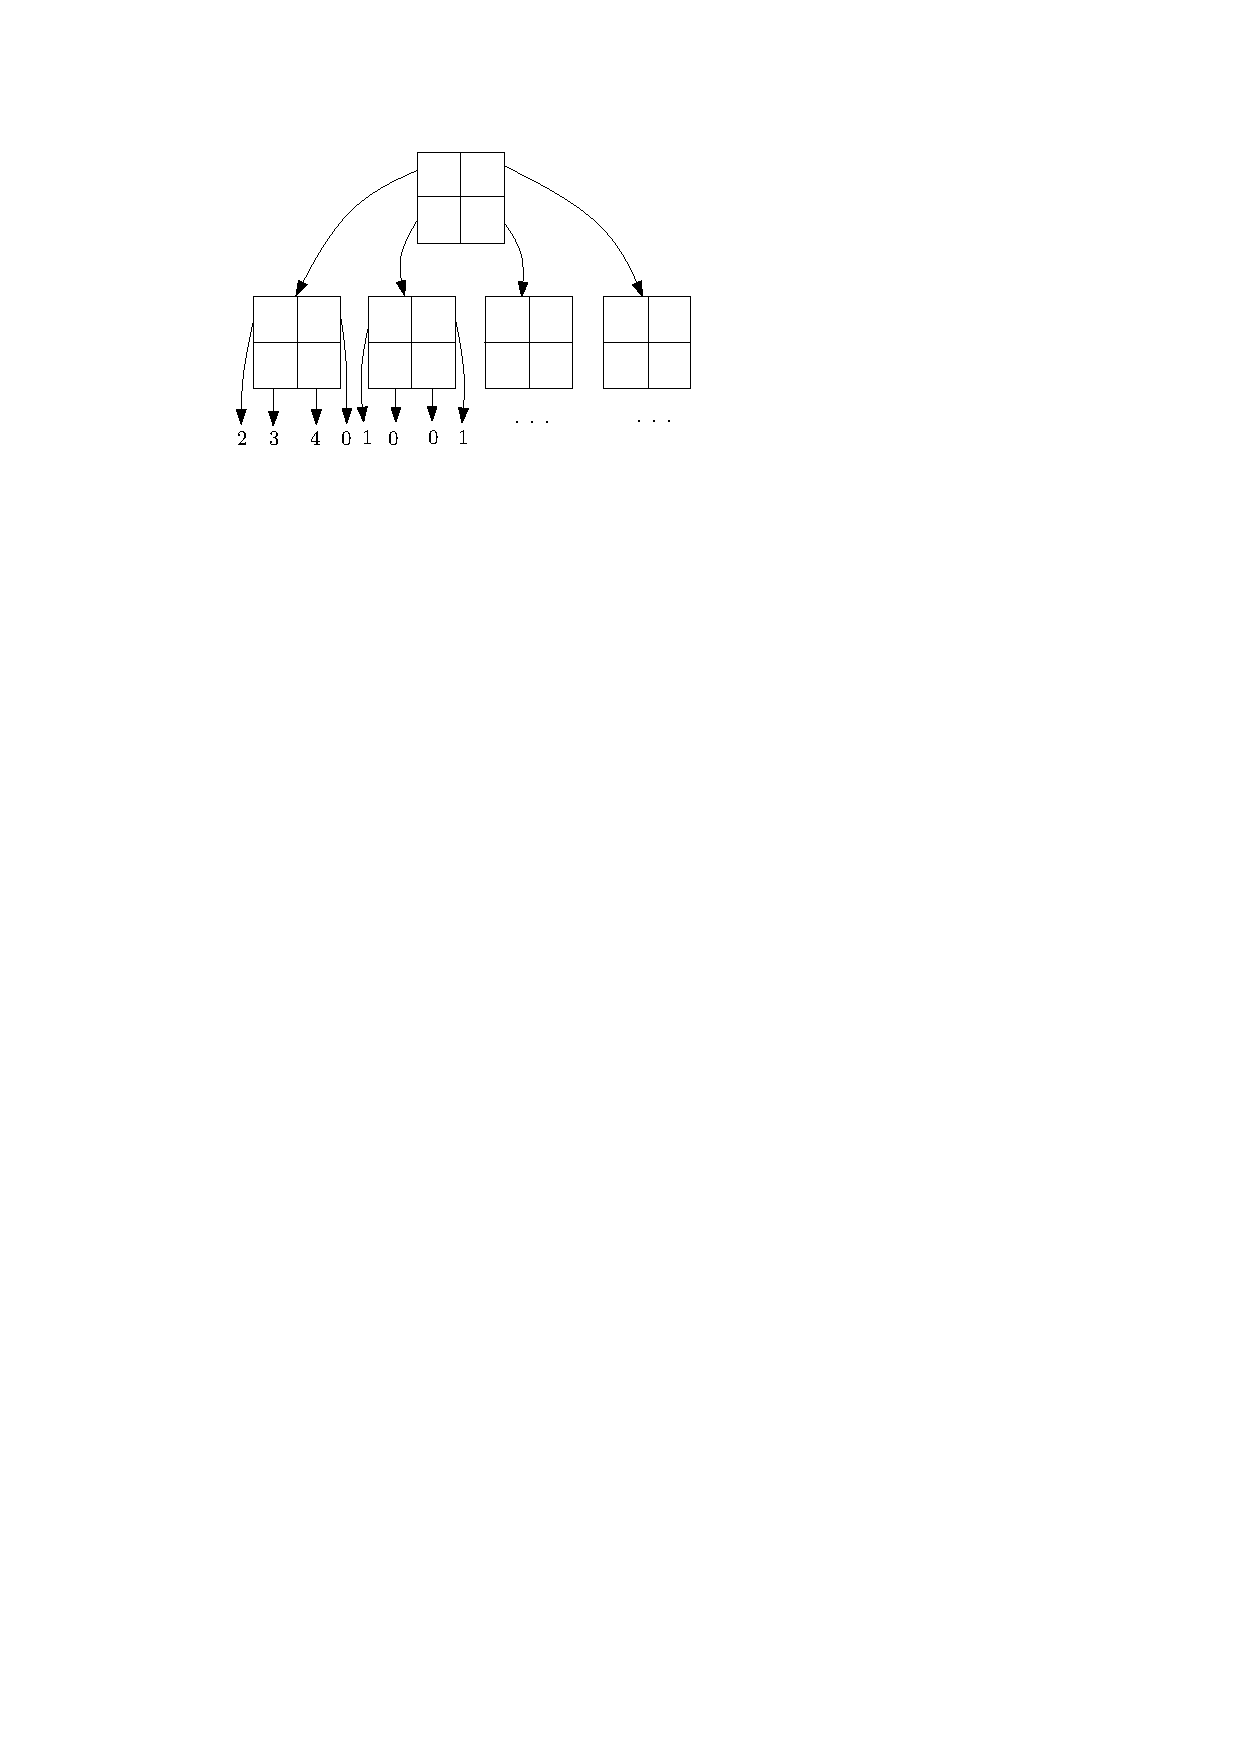
\includegraphics[width=6.0cm]{figures/tree2}\\
\end{subfigure}
\caption{An example of a two-player simultaneous game which has Matching Pennies as a subgame. Each node represents a state of 
the game. Four nodes are shown, and at each node, each player has two individual moves, for the row player: top $t$ and bottom ($b$), 
and for the column player: left ($l$) and right ($r$), leading to four joint moves per node.
\label{fig:example}}
\end{figure}

A {\it matrix game} is a single step simultaneous move game with legal move sets $\cA_1$ and $\cA_2$. 
Each entry in the matrix $A_{rc}$ where $(r,c) \in A_1 \times A_2$ corresponds to a payoff (to player 1) if row $r$ is chosen by 
player 1 (Max) and column $c$ by player 2 (Min). 
For example, in Matching Pennies, each player has two moves. The row player receives a payoff of 1 if both 
players choose the same move and 0 if they do not match. 
Two-player simultaneous move games are sometimes called {\it stacked matrix games} because at every state 
$s$ there is a joint move set $\cA_1(s) \times \cA_2(s)$ that either leads to a terminal state or to a subgame which 
is itself another stacked matrix game. 

A {\it behavioral strategy} for player $i$ is a mapping from states $s \in \cS$
to a probability distribution over the moves $\cA_i(s)$, denoted $\sigma_i(s)$. 
%Given a profile $\sigma = (\sigma_1, \sigma_2)$, define the probability of reaching a terminal state $z$ under $\sigma$ as 
%$\pi^\sigma(z) = \pi_1(z) \pi_2(z) \pi_c(z)$, where each $\pi_i(z)$ is a product of probabilities of the actions taken 
%by player $i$ along the path to $z$ ($c$ being chance's probabilities). 
Define $\Sigma_i$ to be the set of behavioral 
strategies for player $i$. A Nash equilibrium profile in this case is a pair of behavioral strategies optimizing
\begin{equation}\label{eq:ne}
V^* = \max_{\sigma_1 \in \Sigma_1} \min_{\sigma_2 \in \Sigma_2} \bE_{z \sim \sigma}[u_1(z)].
%   = \max_{\sigma_1 \in \Sigma_1} \min_{\sigma_2 \in \Sigma_2} \sum_{z \in Z} \pi^\sigma(z) u_1(z).
\end{equation}
In other words, neither player can improve their utility by deviating unilaterally. 
For example, the Matching Pennies matrix game has a single state and the only equilibrium strategy is to mix equally between both moves, \ie play with a {\it mixed strategy} (distribution) of $(0.5, 0.5)$ giving an expected payoff of $V^* = 0.5$. 
If the strategies also optimize Equation \ref{eq:ne} in each subgame starting in an arbitrary state, the equilibrium strategy is subgame perfect.

In two-player constant-sum games a Nash equilibrium strategy is optimal in the minimax sense. It guarantees the payoff of at least $V^*$ against any opponent. Any 
non-equilibrium strategy has a best response, which will make it win less than $V^*$ in expectation. Moreover, a subgame perfect NE strategy can earn more 
than $V^*$ against weak opponents. After the opponent makes a sub-optimal move, the strategy will never allow it to gain the loss back. 
The value $V^*$ is known as the minimax-optimal value of the game and is the same for every equilibrium profile by von Neumann's minimax theorem.

Two-player constant-sum simultaneous move games can be solved (\ie Nash equilibrium strategies computed) using backward 
induction~\cite{Ross71Goofspiel,Buro03OshiZumo,Rhoads12Computer}. The main idea is to start from the 
endgame positions and individually compute the $V^*$ of each subgame, by solving a linear program at each state, and working back up to the root state.
For the example in Figure 1, the value of the matrix game on the bottom-left is $3$ (if the row player is maximizing) because each player has a 
strategy that is strictly dominated, and the 
value of Matching Pennies is $0.5$. These values represent the unique game-theoretic values for a joint moves $\{ (l,t), (l,b) \}$ in the parent node.
In MCTS, these values are approximated using Monte Carlo sampling, and the variants use the estimates when selecting moves.
As in purely sequential games, search techniques approximate these underlying game-theoretic algorithms, but  
the connection is not as straightforward since the optimal strategies can be mixed and $V^*$ can be anything 
in the range of $[v_{\min}, v_{\max}]$.

%A two-player simultaneous move game is a specific type of two-player imperfect information extensive-form 
%game. In imperfect information games, states are grouped into {\it information sets}: two states $s, s' \in I$ if the player 
%to act at $I$ cannot distinguish which of these states the game is currently in. Any simultaneous move game can be modeled 
%using an information set to represent a half-completed transition, \ie $\cT(s, a_1, ?)$ or $\cT(s, ?, a_2)$. 


The model described above is similar to a two-player finite horizon Markov Game~\cite{Littman94markovgames}.
The model can be easily extended to include chance events~\cite{Lanctot13Goofspiel}. 

\section{Simultaneous Move MCTS}
\label{sec:smmcts}

\newcommand{\SMMCTS}{{\sc SM-MCTS}}
\newcommand{\ExpReq}{{\sc ExpansionRequired}}
\newcommand{\Update}{{\sc Update}}
\newcommand{\Select}{{\sc Select}}
\newcommand{\Playout}{{\sc Playout}}
\newcommand{\Max}{\text{Max}}
\newcommand{\Min}{\text{Min}}


In this section, we present a generalized description of Monte Carlo Tree Search for simultaneous move games. This 
description is based on the one used in Tron~\cite{Perick12Comparison}. First, we describe the overall process. 
Each specific step (\Select, \Update, and final move selection) depends on the chosen variant described in the 
appropriate subsection. The \Update~function is what ensures that rewards are appropriately back-propagated 
to nodes that were visited during the simulation. 

\begin{algorithm2e}[t!]
  \SMMCTS$($node $s$)\\                         \label{alg:function}
  \pushline
    \lIf{$s$ is a terminal state ($s \in \cZ$)}{\Return{$u_1(s)$}}  
    \ElseIf{$s \in T$ {\bf and} \ExpReq$(s)$}{  \label{alg:expand}
      Choose a previously unselected $(a_1,a_2)$ \\
      $s' \gets \cT(s,a_1,a_2)$ \label{alg:choose-expand} \\
      Add $s'$ to $T$\\
      $u_1 \gets$ \Playout($s'$)\\
      $X_{s'} \gets X_{s'} + u_1$ \\    
      $n_{s'} \gets n_{s'} + 1$  \\     \label{alg:increment2}
      \Update$(s, a_1, a_2, u_1)$\\                     \label{alg:update1}
      {\bf return} $u_1$\\
    }                                       
    $(a_1, a_2) \gets $  \Select$(s)$\\        \label{alg:select}
    $s' \gets \cT(s, a_1, a_2)$\\
    $u_1 \gets $ \SMMCTS($s'$)\\                \label{alg:reccall}
    \Update$(s, a_1, a_2, u_1)$ \\                      \label{alg:update2}
    {\bf return} $u_1$\\
  \popline
  \vspace{0.1cm}
  \caption{Simultaneous Move Monte Carlo Tree Search \label{alg:sm-mcts}}
\end{algorithm2e}


In Simultaneous Move MCTS (SM-MCTS), the main difference is that during the selection step, at each node, a {\it joint move}
is selected. The convergence to an 
optimal strategy depends critically on the selection and update policies applied, which are not as straightforward 
as in purely sequential games. 
Algorithm~\ref{alg:sm-mcts} describes a single simulation of SM-MCTS. 
$T$ represents the MCTS tree in which each state is represented by one node. Every node $s$ maintains a 
cumulative reward sum over all simulations through it, $X_s$, and a visit count $n_s$, both initially set to 0. 
As with standard MCTS, when a state is visited these values are incremented on line \ref{alg:increment2}, and in the node 
updates on lines \ref{alg:update1} and \ref{alg:update2}. 
Note that Algorithm~\ref{alg:sm-mcts} explicitly stores the rewards and estimates only in view of player one, 
hence the $u_1$ notation, and the opponent's reward is obtained as $u_2 = k - u_1$ as necessary. 
As seen in Figure~\ref{fig:example}, a matrix of references to the children is maintained at each state. 

At node $s$, the estimated values $\bar{X}_{s'}$ of the children nodes $s' = \cT(s,a_1,a_2)$ over all 
joint moves form an estimated payoff matrix for node $s$. 
The critical parts of the algorithm are the updates on lines \ref{alg:update1} and \ref{alg:update2}, and the selection 
on line \ref{alg:select}. 
Each variant below will describe a different way to select a joint move and update a node. 

% MarcL, Mar27: Removed since we're not including any of these 
%In practice, there are several optimizations to the base algorithm that might be desirable.
%If a game has a large branching factor, it may take many iterations for 
%the expansion condition and consequence in lines \ref{alg:expand} to \ref{alg:choose-expand} to fill up the matrix before 
%switching to a selection policy. 
%The matrix can instead be filled such that at least one action has been taken from each row and one from each column before 
%switching to the selection policy. 
%Since most variants do not require values for each entry in the matrix, this could reduce the number of simulations before 
%switching to $|\cA_1(s)| + |\cA_2(s)|$ from $|\cA_1(s)||\cA_2(s)|$. The use of progressive 
%widening~\cite{Chaslot08Progressive} may also lead to deeper searches. 
%In this paper, the implementation for experiments is based on the pseudo-code presented in Algorithm~\ref{alg:sm-mcts}.

We focus on a number of SM-MCTS variants. The most popular one is straightforward adaption of UCT. 
Though it has been shown to not converge to a Nash equilibrium even in a one-shot single-state 
game, it has nonetheless been popular and successful in general game playing~\cite{Shafiei09}. 
The second is Exp3, an regret minimization algorithm that can be used to learn in unknown games
games~\cite{Exp3}, was also applied successfully to the popular online card game Urban Rivals~\cite{Teytaud11Upper,StPierre12Online}. 
The third is Regret Matching, which was recently shown to perform particularly well in Goofspiel~\cite{Lanctot13Goofspiel}.
The latter two were also used in a recent theoretical analysis of the convergence of SM-MCTS~\cite{Lisy13Computing}.
Finally, we also try Sequential UCT, which has been previously used in Tron~\cite{Samothrakis10Tron,Lanctot13Tron}.

\subsection{Decoupled UCT} 

In Decoupled UCT (DUCT), each player $i$ maintains for every state $s$ separate reward sums $X^i_{s,a}$ and 
visit counts $n^i_{s,a}$ for their own move set $a \in \cA_i(s)$. 
In essence, each player {\it decouples} the matrix in each state and applies UCB over the cumulative rewards for 
each of their own move as if there was no joint dependency on these rewards.
When a joint move needs to be selected on line 
\ref{alg:select}, each player selects a move that maximizes the decoupled UCB value over their reward estimates 
independently:
\begin{equation}
\label{eq:duct}
a_i = \argmax_{a \in \cA_i(s)}{ \left\{ \bar{X}^i_{s,a} + C \sqrt{\frac{\ln n_s}{n_{s,a}}} \right\} }, 
  \mbox{ where } \bar{X}^i_{s,a} = \frac{X^i_{s,a}}{n_{s,a}}
\end{equation}
\noindent Here, $C$ is a parameter that determines how much weight to place on exploration. 
In DUCT, \Update~simply increments the decoupled values for each player $i$: $X^i_{s,a_i} \leftarrow X^i_{s,a_i} + u_i$,
and $n_{s,a_i} \leftarrow n_{s,a_i} + 1$. 

As an example, consider the game in Figure~\ref{fig:example}, with player set $\cN = \{\Max,\Min\}$, root node $s$,
and move sets $\cA_{\Max}(s) = \{t,b\}, \cA_{\Min}(s) = \{l,r\}$.  
Suppose four simulations are run, and rewards received are $u_\Max = 3$ for $(t,l)$, $2$ for $(t,r)$, $1$ for $(b,l)$, 
and $0$ for $(b,r)$. The tree would contain exactly five states: $s$, and each child of $s$. On the fifth simulation, 
\Max~chooses among $t$ and $b$ and \Min~chooses among $r$ and $l$, both by using Equation~\ref{eq:duct}. 
In this case, $\bar{X}_{s,t}^\Max = (3 + 2) / 2 = 2.5$ and $\bar{X}_{s,b}^\Max = (1 + 0) / 2 = 0.5$. 
Supposing $v_{\max} = 4$, then $\bar{X}_{s,l}^\Min = (1 + 3) / 2 = 2$ and $\bar{X}^\Min_{s,r} = (2 + 4) / 2 = 3$. 

In DUCT, after all the simulations have been performed, each player $i$ chooses separately their own final move 
with the highest estimated reward $\max_{a \in \cA_i(s)} \bar{X}^i_{s,a}$. 

\subsection{Exp3}

In Exp3~\cite{Exp3}, each player maintains an estimate of the sum of rewards, denoted $\hat{x}^i_{s,a}$, and visit 
counts $n^i_{s,a}$ for each of their own moves. In the case of Exp3, however, $\hat{x}^i_{s,a}$ represents a cumulative 
{\it weighted} reward, where each value gets scaled by the probability of it having been sampled. 
These values and strategies are maintained separately for each player, so Exp3 is decoupled in the same sense as DUCT. 

The joint move selected on line \ref{alg:select} is composed of moves independently selected for each player 
based on a sampling probability distribution composed for each player based on $\hat{x}^i_{s,a}$. 
The probability of sampling move $a_i$ is
\begin{equation}
\label{eq:exp3select}
\sigma^t_i(s,a_i) = \frac{(1-\gamma) e^{\eta w^i_{s,a_i}}}{\sum_{a_j \in \cA_i(s)} e^{\eta w^i_{s,a_j}}} + \frac{\gamma}{|\cA_i(s)|}, \mbox{ where }
\end{equation}
\[ \eta = \frac{\gamma}{|\cA_i(s)|}, \mbox{ and } w^i_{s,a} = \hat{x}^i_{s,a} - \max_{a' \in \cA_i(s)} \hat{x}^i_{s,a'}. \]

\noindent Here, $\gamma$ is the probability of exploring (choosing a random move). 
The update after selecting joint move $(a_1,a_2)$ and obtaining a simulation result $(u_1,u_2)$ updates the visits count 
and adds to the corresponding reward sum estimates the reward divided by the probability that the move was played by the player using
$n_{s,a_i} \leftarrow n_{s,a_i} + 1, \hat{x}^i_{s,a_i} \leftarrow \hat{x}^i_{s,a_i} + \frac{u_i}{\sigma^t_i(s,a_i)}$.
Dividing the value by the probability of selecting the corresponding move makes $\hat{x}^i_{s,a}$ estimate the sum of rewards over all 
iterations, not only the ones where $a_i$ was selected. 

The mixed strategy used by player $i$ after the simulations are done is given by the frequencies of visit counts of the moves, 
$\sigma^{final}_i(s,a_i) =  n_{s,a_i}~/~\sum_{b_i\in A_i(s)} n_{s,b_i}$.
Previous work \cite{Teytaud11Upper} suggests first removing the samples caused by the exploration. This modification proved to be useful also in our experiments, so before computing the resulting final mixed strategy, we set
\begin{equation}
n_{s,a_i}' \leftarrow \max\left(0,n_{s,a_i} - \frac{\gamma}{|A_i(s)|}\sum_{b_i\in A_i(s)}n_{s,b_i}\right).
\end{equation}
For final move selection, a move is chosen by sampling according to a distribution that normalizes $n'_{s,a_i}$. 

\subsection{Regret Matching}

This variant applies regret matching \cite{Hart00} to the current estimated matrix game at each stage. 
Suppose iterations are numbered from $t \in \{ 1, 2, 3, \cdots \}$ and at each iteration and each node $s$ 
there is a mixed strategy $\sigma_i^t(s)$ used by each player $i$ for each node $s$ in the tree, initially set to 
uniform random: $\sigma^0_i(s,a) = 1 / |\cA(s)|$. 
Each player $i$ maintains a cumulative regret $r^i_s[a]$ for having played $\sigma_i^t(s)$ instead of $a \in \cA_i(s)$. 
In addition, a table for the average strategy is maintained per player as well $\bar{\sigma}^i_s[a]$. The values in 
both tables are initially set to 0. 
As in DUCT, the regret values $r^i_s[a_i]$ are maintained separately by each player.
However, the updates and specifically the reward uses a value that is a function of the joint move space. 

On iteration $t$, the selection policy (line \ref{alg:select} in Algorithm~\ref{alg:sm-mcts}) first builds 
the player's current strategies from the cumulative regret. Define the operator $(\cdot)^+ = \max(\cdot,0)$, 
\ie $(-3)^+ = 0$ and $4^+ = 4$, and define
\begin{equation}
\label{eq:rm}
\sigma^t_i(s,a) = \frac{r^i_s[a]}{R^+_{sum}} \mbox{ if } R^+_{sum} > 0 \mbox{ or } 
\frac{1}{|\cA_i(s)|} \mbox{ otherwise},
\end{equation}
where $R^+_{sum} = \sum_{a \in \cA_i(s)}{r^{i,+}_s[a]}$. 
The main idea is to adjust the strategy by assigning higher weight proportionally to moves based on the regret of 
having not taken them over the long-term. 
To ensure exploration, a $\gamma$-on-policy sampling procedure similar to Equation~\ref{eq:exp3select} is used 
choosing move $a$ with probability $\gamma/|\cA(s)| + (1-\gamma) \sigma^t_i(s,a)$. 

The updates on line \ref{alg:update1} and \ref{alg:update2} add regret accumulated at the iteration to  
the regret tables $r^i_s$ and the average strategy $\bar{\sigma}^i_s[a]$. 
Suppose joint move $(a_1,a_2)$ is 
sampled from the selection policy and utility $u_i$ is returned from the recursive call on line~\ref{alg:reccall}. 
Label the current child $(i,j)$ estimate $\bar{X}_{s,i,j}$ and the $reward(i,j) = \bar{X}_{s,i,j}$ if 
$(i,j) \not= (a_1,a_2)$, or $u_i$ otherwise. The updates to the regret are:
\begin{eqnarray*}
\forall a_1' \in \cA_1(s),  r^1_s[a_1'] \leftarrow r^1_s[a_1'] + ( reward(a_1', a_2) - u_1 ),\\
\forall a_2' \in \cA_2(s),  r^2_s[a_2'] \leftarrow r^2_s[a_2'] + ( reward(a_1, a_2') - u_2 ),
\end{eqnarray*}
\noindent and average strategy updates are $\bar{\sigma}^i_s[a] \leftarrow \bar{\sigma}^i_s[a] + \sigma^t_i(s,a)$ 
for each player. Here, $u_1$ is the reward for player one and recall that the reward for the other player $u_2 = k - u_1$.

The final move for the root $s$ is chosen by sampling over the strategy obtained by 
normalizing the values in $\bar{\sigma}_s^i$. 

\subsection{Sequential UCT}

Sequential UCT (SUCT) performs regular UCT on a {\it serialized} game tree, \ie one that is turned into a 
purely sequential game. 

Recall again the simultaneous move game from Figure~\ref{fig:example}. If the row 
player always chooses ``top'' $(t)$ and the column player always chooses ``left'' $(l)$, then in the simultaneous 
move MCTS, the simulation would consist of two joint moves, $(t,l) \rightarrow (t,l) \rightarrow 2$. However, 
in SUCT, this simulation would be four steps. First, the searching player chooses $t$, then it becomes the opponent's
turn and responds with $l$, then the player plays $t$ again, and the opponent again responds with $l$.  

Therefore, In SUCT a different tree is built, one where a player chooses a move and the opponent is 
allowed to know which move the player chose and can respond accordingly. The motivation for this is that if a player
announces his move to the opponent and the opponent is allowed to choose a 1-ply best response, then the searching player
will learn to play the move that has the least chances of being penalized by an opponent. In fact, in the classic 
minimax setting, the values returned by a search of the serialized game tree are indeed bounds on the actual true 
minimax value of the node~\cite[Corollary 4.2]{Bosansky13Using}, so it seems reasonable in the SM-MCTS setting as well. 

In this paper, we assume that the searching player always moves first and then the opponent responds, leading to 
defensive play. However, in general this could be could be reversed for aggressive play, or even randomized as was 
done in $\alpha\beta$ search for abstract combat games~\cite{Kovarsky05RAB}.

%\section{Application to General Game-Playing}
%\label{sec:appggp}
%\subsection{Using N-Grams for Dynamic Playout Policies}

\section{Empirical Evaluation}
\label{sec:exp}

In this section, we discuss our experimental setup for evaluation SM-MCTS to in general games.
We start by describing nine simultaneous move games used previously in GGP. Some of these 
descriptions are taken from~\cite[Appendix C]{Finnsson12}.

%An interesting challenge in GGP is the efficient parsing and logical interpretation of the game rules. 
%Since this paper focuses on the search algorithm variants and their performance, our implementation 
%does not explicitly interpret the rules from logical descriptions. However care has been taken to 
%ensure that none of the algorithms benefit from domain knowledge. 

\subsection{Game Descriptions}
\label{subsec:games}

\textit{Battle} is played on an 8$\times$8 board. Each player has 20 disks. These disks can move one square or 
capture an opponent square next to them. Instead of a move, the player can choose to defend a square occupied by their 
piece. If an attacker attacks such a defended square, the attacker will be captured. The goal is to be the first player 
to capture 10 opponent disks. 

\textit{Bidding Tic-Tac-Toe} is a variation of normal Tic-Tac-Toe where there is a bidding round between 
normal play that decides who gets to place a marker on the board. Each player begins with three coins, and the 
\textsc{x} player has an additional tiebreaker token. When a player wins a bidding round, allowing that player to 
place a marker, the coins used to bid are given to the opponent. The tiebreaker token can optionally be used to break 
ties, and if so, the tiebreaker token is also given to the opponent. The winning conditions are the same as 
standard Tic-Tac-Toe. 

\textit{Chinook} is a variant of \textit{Breakthrough} where two independent games are played simultaneously. 
One game on the white squares and another one on the black squares. Black and White move their pieces simultaneously 
like Checkers pawns. As in Breakthrough, the first player that reaches the opposite side of the board wins the game. 

\textit{Goofspiel}$(N)$ is a card game where each player gets $N$ cards marked 1-$N$, and there is a central pile, 
shuffled and face down called the point-card deck (also 1-$N$). Every turn, the top card of this point card deck flips, 
it is called the {\it upcard}. Then, players choose a {\it bid} card from their hand and reveal it simultaneously. 
The player with the higher bid card obtains a number of points equal to the value of the upcard. The bid cards and 
upcard are then discarded and a new round starts. At the end of $N$ rounds, the player with the highest number of 
points wins. If the number of points are tied, the game ends in a draw. The standard game of Goofspiel has 
$N = 13$. In this paper, we assume that the point cards have a fixed order. 

In \textit{Runners} each turn both players decide how many steps they want to move forward or backward. The aim 
is to reach the goal location before the opponent does.

\textit{Oshi-Zumo}$(N,K,M)$ is a wrestling simulation game played on a discrete single-dimensional grid with 
$2K+1$ positions, where each player starts with $N$ coins~\cite{Buro03OshiZumo}. A wrestler token begins in the middle 
position. Every turn, 
each player bids $b \ge M$ coins. The coins bid are then discarded and the player bidding the most coins pushes the 
wrestler one position closer to the goal for that player. 

\textit{Pawn Whopping} is a simultaneous move version of Breakthrough, played on an 8 $\times$ 8 board. Each player has 
16 pawns starting on one side of the board and the goal is to move one of their pieces to the other side of the board. 
Pawns can capture diagonally and only move forward one cell straight or diagonally.
If opposing pawns try to capture each other or move to the same square, no change is made. 
Pawn Whopping has slightly different movement and is simultaneous.

\textit{Racetrack Corridor} is played on a board with length 5 cells and width 3 cells. Each player starts at the top of the board and the aim is to reach the other side of the board before the opponent does. Each move, the player can decide to move forward, sideways or place a wall on the board of the opponent which spans two thirds of the width of the board.

\textit{Tron} is a two-player game played on discrete two-dimensional grid possibly obstructed by walls. At each
step in Tron both players move to adjacent cells, and a wall is placed in the cells that the player started on that turn. 
The game is won if the opponent crashes into a wall or moves off the board. If both players crash at the same turn 
into a wall, the game ends in a draw. The initial position is a 13 $\times$ 13 square field walled ``box'' in the 
center (board (a) from \cite{Lanctot13Tron}). 

\subsection{Test Environment}

Each of the games described above is implemented in Java. As we intend for our comparison to be general, the domains were 
influenced by those used in GGP competitions and research work, and our goals are to closely match the conditions of the 
GGP settings. 
The advantage is that we do not have to deal with a slow GDL reasoner. Therefore, we can use shorter time settings than 
the longer time settings which are used more often in GGP, and still guarantee more simulations. Only the rules of the 
games are implemented without any domain knowledge. Therefore every variant uses a uniform random playout policy. 
In this way, we still mimic GGP, but this setup allows to perform 
the experiments much faster and generate far more games to ensure the assessments are based on data that is statistically
significant. 

DUCT, SUCT, Exp3, and RM are pair wise compared in each of the nine games. The time setting is 2.5 seconds per move and 
each combination of one variant versus another in a particular game consists of 500 games.  

In GGP, all utilities are non-negative, so without loss of generality, $u_1, u_2 \ge 0$.  
Also, games may not be constant-sum. In our implementation, we ensure that all payoffs 
are appropriately scaled to ensure that they are $k$-sum, with $k > 0$, by using 
a similar transformation previously used in \Cadiaplayer~\cite{Finnsson12}:
\[ \text{\sc Scale}(u_1, u_2) = \left( \frac{u_1 - u_2 + k}{2}, \frac{u_2 - u_1 + k}{2} \right). \]

\subsection{Parameter Tuning}

\begin{table}[t!]
\centering
\begin{tabular}{|c|c|c|c|c|}
\hline
                  & DUCT    & SUCT    & Exp3           & RM  \\
\hline
Battle            & $C=0.0$ & $C=0.4$ & $\gamma = 0.8$ & $\gamma = 0.10$  \\ 
BiddingTicTacToe  & $C=0.0$ & $C=0.0$ & $\gamma = 0.9$ & $\gamma = 0.15$   \\ 
Chinook           & $C=0.4$ & $C=0.4$ & $\gamma = 0.2$ & $\gamma = 0.30$ \\ 
Goofspiel         & $C=0.4$ & $C=0.8$ & $\gamma = 0.1$ & $\gamma = 0.20$ \\ 
Oshi-Zumo         & $C=0.4$ & $C=1.8$ & $\gamma = 0.6$ & $\gamma = 0.75$ \\ 
PawnWhopping      & $C=0.0$ & $C=0.4$ & $\gamma = 0.4$ & $\gamma = 0.75$  \\ 
RacetrackCorridor & $C=1.2$ & $C=0.8$ & $\gamma = 0.4$ & $\gamma = 0.15$\\ 
Runners           & $C=0.8$ & $C=1.8$ & $\gamma = 0.3$ & $\gamma = 0.50$ \\
Tron              & $C=1.8$ & $C=2.0$ & $\gamma = 0.3$ & $\gamma = 0.30$ \\
 \hline
\end{tabular}
\caption{Parameters values. \label{tbl:parameters}}
\end{table}


Before the different algorithms are compared, their parameters are tuned by self-play where different parameter 
values are compared against a reference parameter. In DUCT, and SUCT the default parameter is $C=1.4$. The reference
parameters for Exp3 and RM are set to $\gamma = 0.2$ and $\gamma = 0.025$, respectively, because they are the optimal 
parameters in Goofspiel \cite{Lanctot13Goofspiel}. The tuned parameter values are shown in Table \ref{tbl:parameters}. 

The table shows that the optimal parameter value depends on the game. As it is difficult to choose one parameter value 
for each algorithm that works well in all games, we choose to use a different parameter value for each game separately. 
In this way, we can see how well each of the algorithms can perform under optimal conditions. In the GGP context 
this is difficult, because the game playing agents often have severely restricted time to interpret the 
rules before play starts. 

\begin{figure*}[t!]
\centering
\begin{tabular}{ccc}
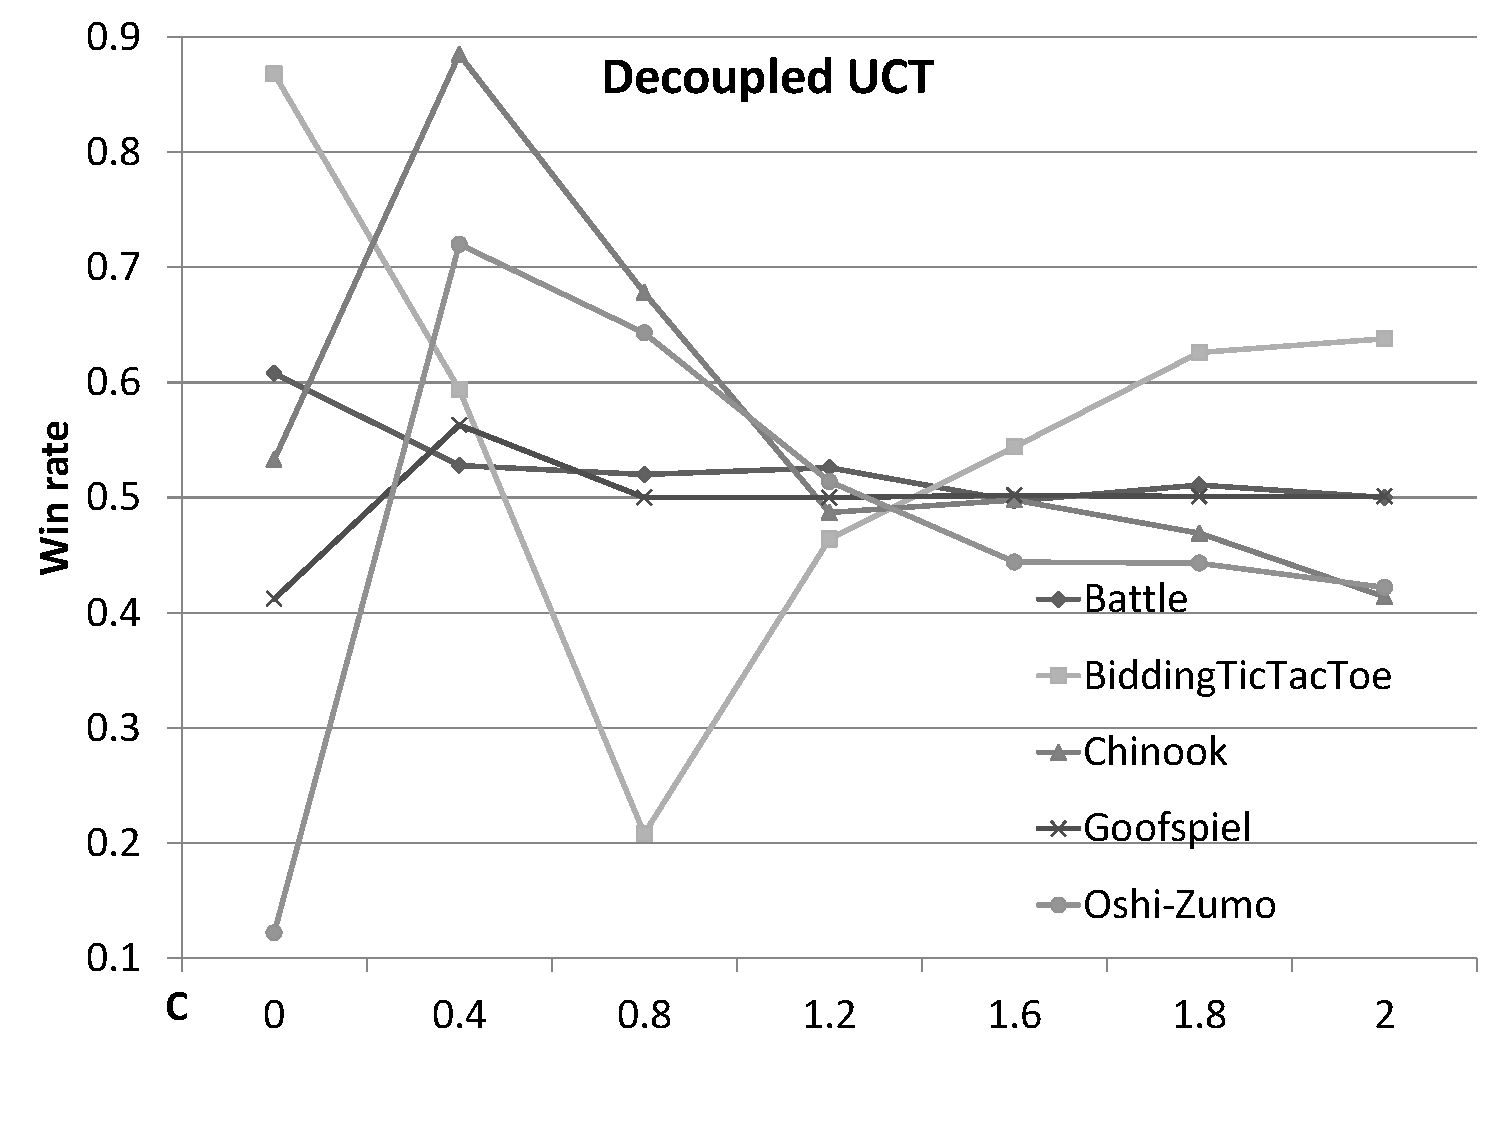
\includegraphics[scale=0.3]{figures/duct1} & ~ & 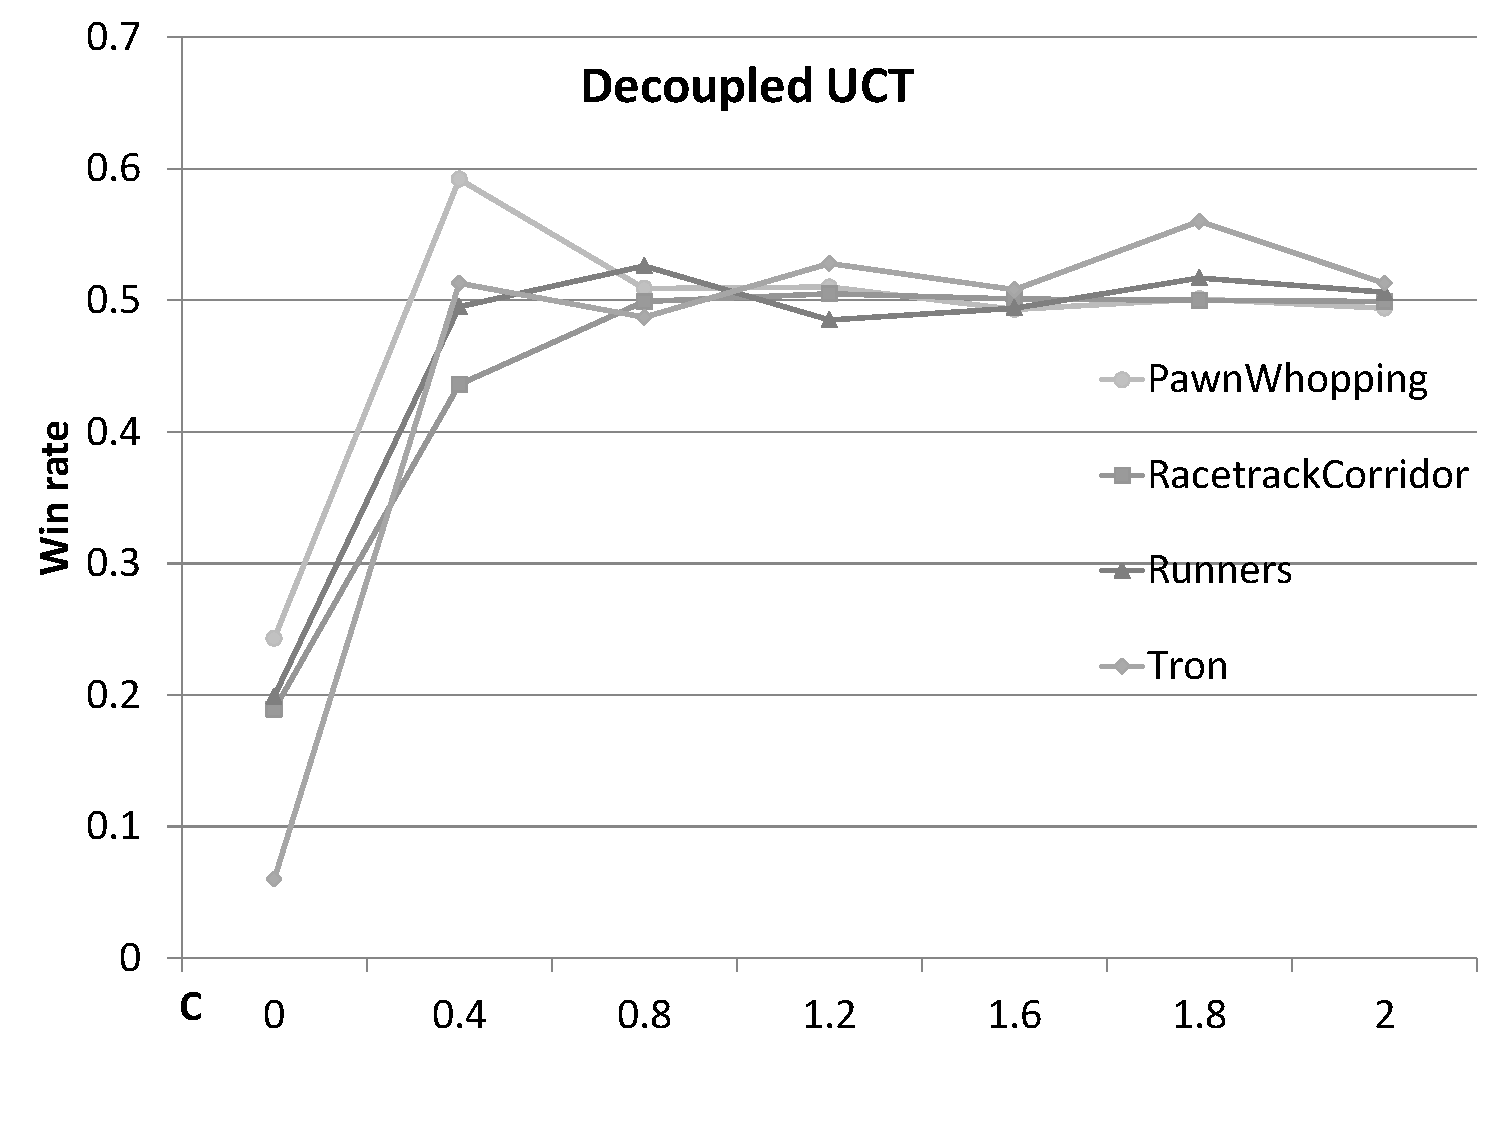
\includegraphics[scale=0.3]{figures/duct2}\\
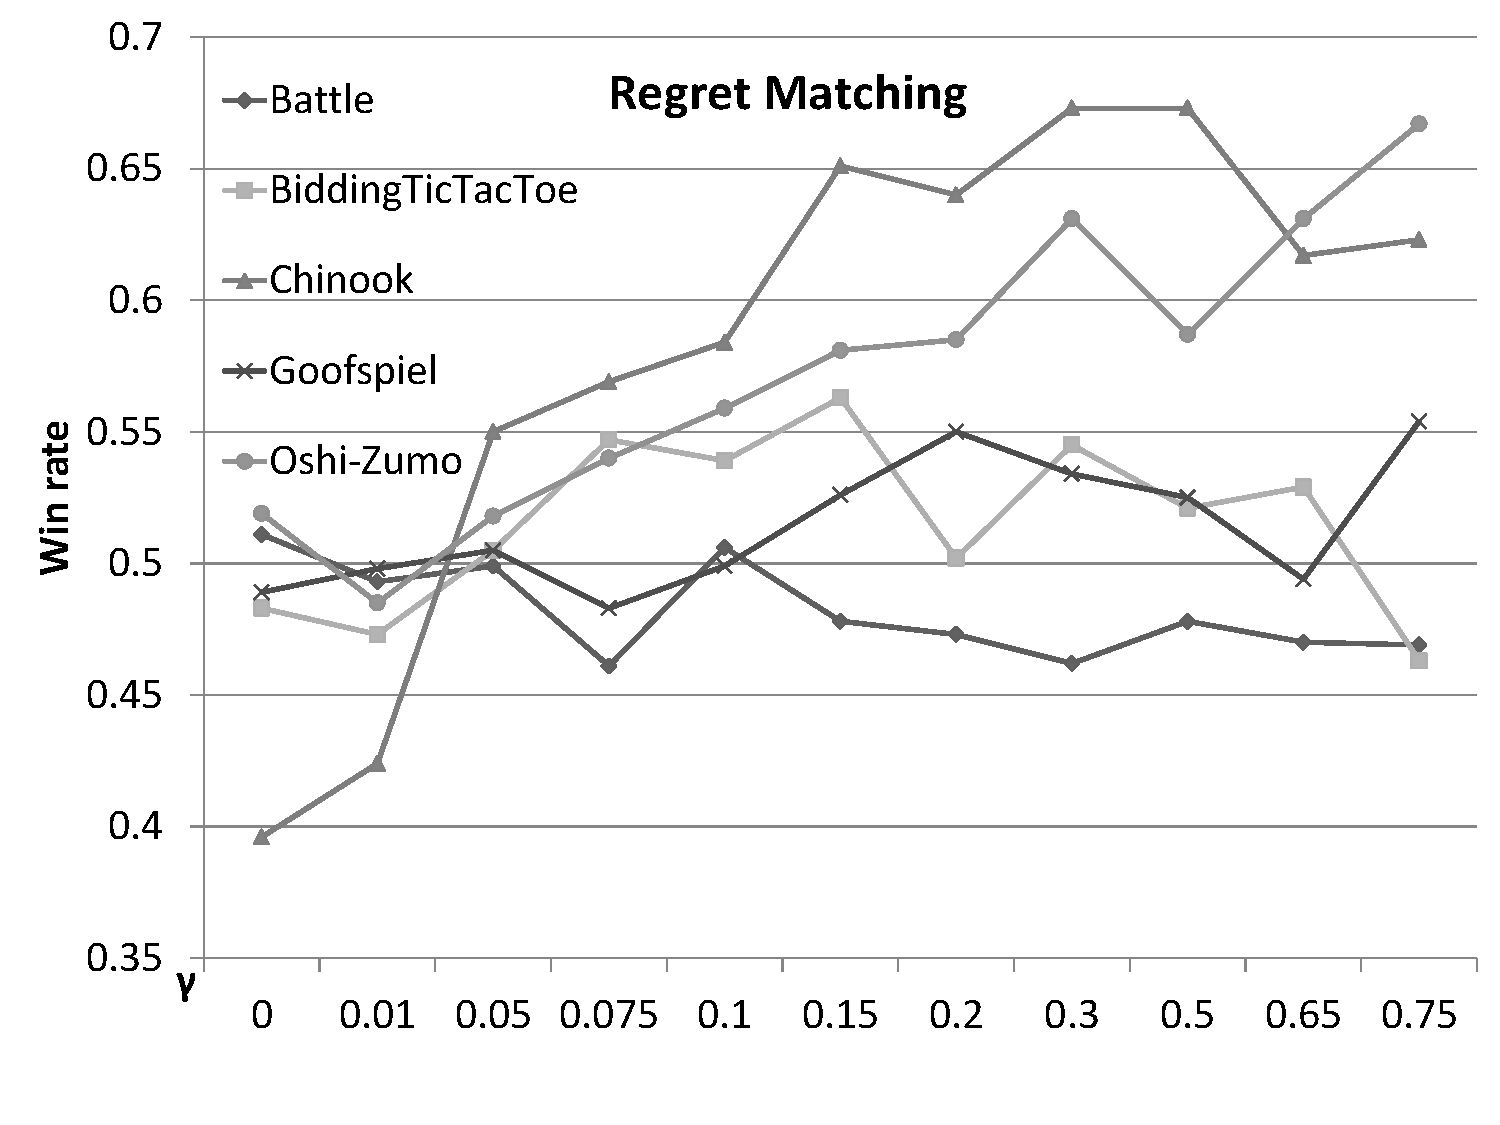
\includegraphics[scale=0.3]{figures/regretmatching1} & ~ & 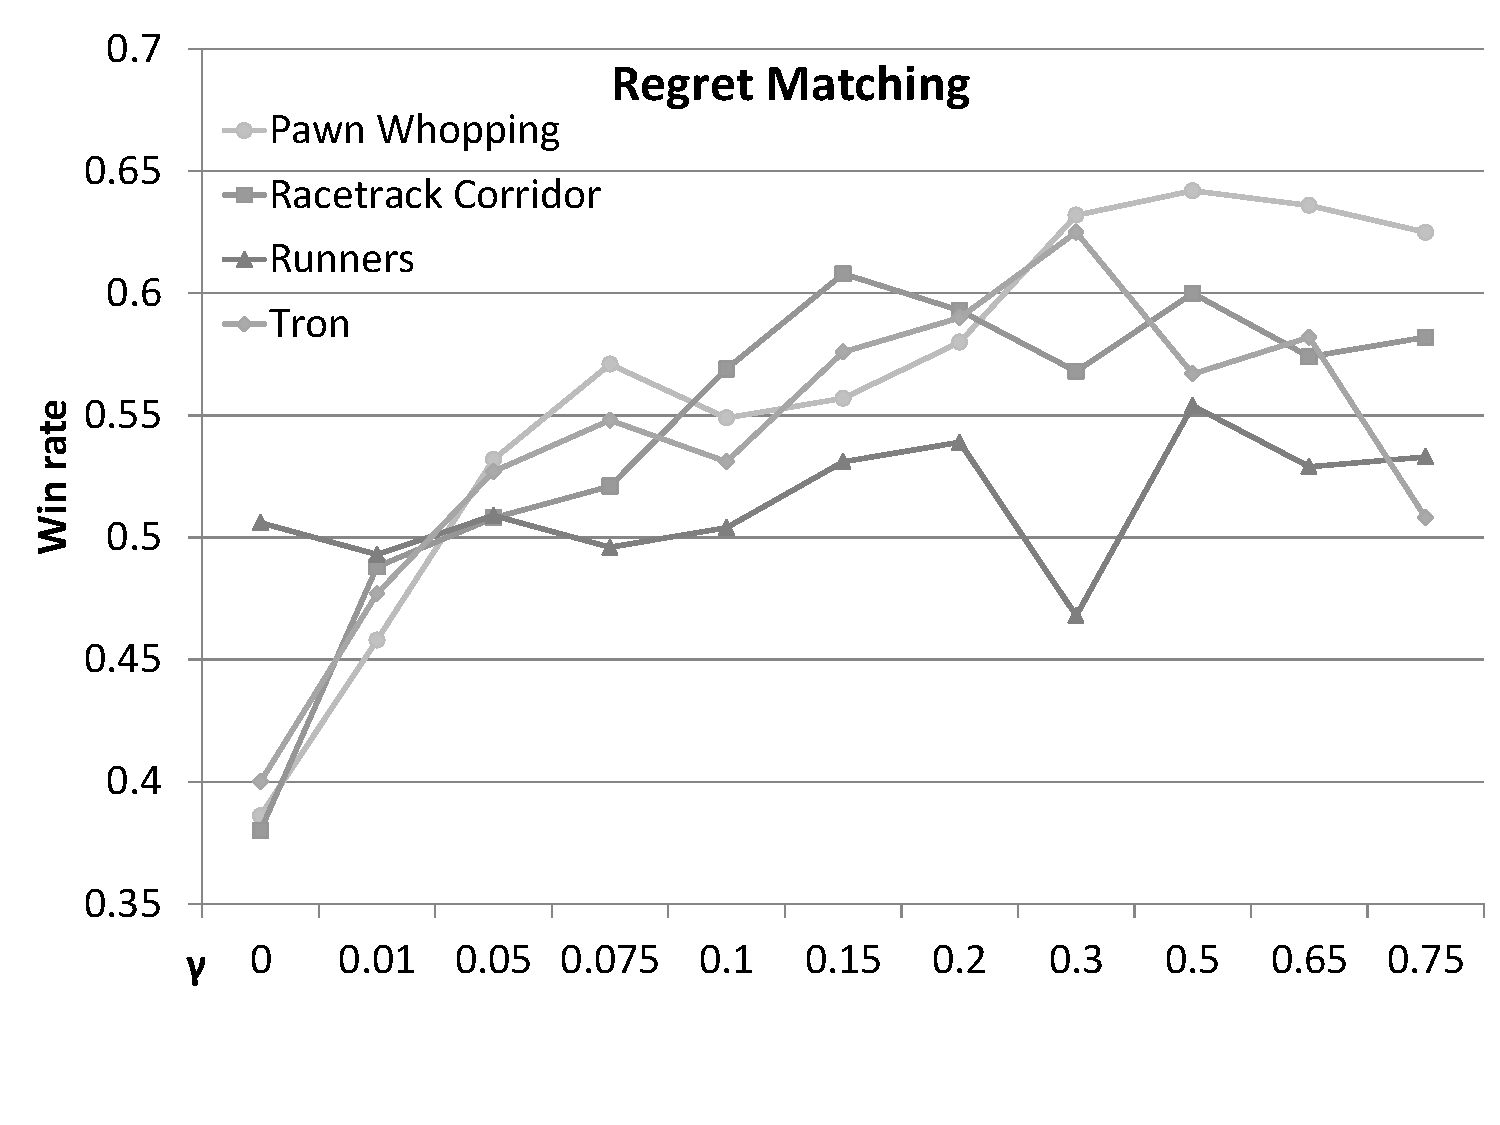
\includegraphics[scale=0.3]{figures/regretmatching2}\\
\end{tabular}
\caption{Tuning Regret Matching and Decoupled UCT}
\label{fig:tuning1}
\end{figure*}

\subsection{Experimental Results}
\label{subsec:results}

In this subsection, we present and discuss the results of our experiments. 

\subsubsection{Parameter Landscape}

Figure \ref{fig:tuning1} shows the win rate of Decoupled UCT depending on $C$ against the reference parameter $C=1.4$ and 
shows the win rate of Regret Matching depending on $\gamma$ against the reference parameter $\gamma = 0.025$. The figure 
highlights two important results. First, it is not possible to choose a parameter value that performs well in all games. 
Second, the performance of Regret Matching and Decoupled UCT can depend heavily on the corresponding parameter value. 

We notice that the win rates of DUCT vary quite sensitively in BiddingTicTacToe, Oshi-Zumo, and Chinook, and even more so when $C < 1.2$. 
For Regret Matching, generally interval $\gamma \in [0.2,0.5]$ seems to be save but the optimal parameter varies significantly across game types.

This kind of behavior also holds for the other algorithms. Therefore, this figure supports choosing a separate parameter value 
for each game and algorithm. See Table~\ref{tbl:parameters} for the chosen parameter values.

% MarcL, Mar. 27th: I took this out of the intro as it was too specific. Maybe we can discuss it here at some point.
%Unlike in \cite{Samothrakis10Tron}, they found that {\it UCB1-Tuned} was the most successful in Tron, 
%which was also confirmed by a more recent study~\cite{Lanctot13Tron}.

\subsubsection{Performance Comparisons}

\begin{table}
\begin{center}
\begin{tabular}{|c|rrrr|}
\hline
         Battle    &       DUCT   &       Exp3   &         RM   &       SUCT   \\
\hline
           DUCT    &          & 74.90 ($\pm$ 2.19)   & 74.30 ($\pm$ 2.24)   & 55.40 ($\pm$ 2.99)   \\
           Exp3    & 25.10 ($\pm$ 2.19)   &          & 42.60 ($\pm$ 2.80)   & 25.00 ($\pm$ 2.19)   \\
             RM    & 25.70 ($\pm$ 2.24)   & 57.40 ($\pm$ 2.80)   &          & 25.00 ($\pm$ 2.19)   \\
           SUCT    & 44.60 ($\pm$ 2.99)   & 75.00 ($\pm$ 2.19)   & 75.00 ($\pm$ 2.19)   &          \\
\hline
\hline
B.T.T.T.   &       DUCT   &       Exp3   &         RM   &       SUCT   \\
\hline
           DUCT    &          & 64.10 ($\pm$ 4.06)   & 51.80 ($\pm$ 4.29)   & 53.80 ($\pm$ 4.16)   \\
           Exp3    & 35.90 ($\pm$ 4.06)   &          & 46.10 ($\pm$ 4.32)   & 38.80 ($\pm$ 4.11)   \\
             RM    & 48.20 ($\pm$ 4.29)   & 53.90 ($\pm$ 4.32)   &          & 47.00 ($\pm$ 4.28)   \\
           SUCT    & 46.20 ($\pm$ 4.16)   & 61.20 ($\pm$ 4.11)   & 53.00 ($\pm$ 4.28)   &          \\
\hline
\hline
        Chinook   &       DUCT   &       Exp3   &         RM   &       SUCT   \\
\hline
           DUCT    &          & 92.90 ($\pm$ 2.23)   & 99.80 ($\pm$ 0.39)   & 68.50 ($\pm$ 4.04)   \\
           Exp3    & 7.10 ($\pm$ 2.23)   &          & 91.50 ($\pm$ 2.42)   & 18.90 ($\pm$ 3.41)   \\
             RM    & 0.20 ($\pm$ 0.39)   & 8.50 ($\pm$ 2.42)   &          & 2.30 ($\pm$ 1.30)   \\
           SUCT    & 31.50 ($\pm$ 4.04)   & 81.10 ($\pm$ 3.41)   & 97.70 ($\pm$ 1.30)   &          \\
\hline
\hline
      Goof         &       DUCT   &       Exp3   &         RM   &       SUCT   \\
\hline
           DUCT    &          & 46.00 ($\pm$ 3.61)   & 4.90 ($\pm$ 1.88)   & 75.10 ($\pm$ 3.37)   \\
           Exp3    & 54.00 ($\pm$ 3.61)   &          & 37.90 ($\pm$ 4.23)   & 60.40 ($\pm$ 3.92)   \\
             RM    & 95.10 ($\pm$ 1.88)   & 62.10 ($\pm$ 4.23)   &          & 30.20 ($\pm$ 4.01)   \\
           SUCT    & 24.90 ($\pm$ 3.37)   & 39.60 ($\pm$ 3.92)   & 69.80 ($\pm$ 4.01)   &          \\
\hline
\hline
       O.Z.   &       DUCT   &       Exp3   &         RM   &       SUCT   \\
\hline
           DUCT    &          & 81.50 ($\pm$ 2.65)   & 30.60 ($\pm$ 3.74)   & 79.70 ($\pm$ 2.72)   \\
           Exp3    & 18.50 ($\pm$ 2.65)   &          & 23.50 ($\pm$ 3.45)   & 34.30 ($\pm$ 3.50)   \\
             RM    & 69.40 ($\pm$ 3.74)   & 76.50 ($\pm$ 3.45)   &          & 65.10 ($\pm$ 3.87)   \\
           SUCT    & 20.30 ($\pm$ 2.72)   & 65.70 ($\pm$ 3.50)   & 34.90 ($\pm$ 3.87)   &          \\
\hline
\hline
   P.W.   &       DUCT   &       Exp3   &         RM   &       SUCT   \\
\hline
           DUCT    &          & 72.60 ($\pm$ 3.01)   & 97.90 ($\pm$ 1.11)   & 61.20 ($\pm$ 3.36)   \\
           Exp3    & 27.40 ($\pm$ 3.01)   &          & 95.30 ($\pm$ 1.72)   & 48.00 ($\pm$ 3.85)   \\
             RM    & 2.10 ($\pm$ 1.11)   & 4.70 ($\pm$ 1.72)   &          & 17.10 ($\pm$ 3.17)   \\
           SUCT    & 38.80 ($\pm$ 3.36)   & 52.00 ($\pm$ 3.85)   & 82.90 ($\pm$ 3.17)   &          \\
\hline
\hline
R.C.   &       DUCT   &       Exp3   &         RM   &       SUCT   \\
\hline
           DUCT    &          & 60.40 ($\pm$ 1.93)   & 98.40 ($\pm$ 0.77)   & 49.90 ($\pm$ 0.65)   \\
           Exp3    & 39.60 ($\pm$ 1.93)   &          & 93.70 ($\pm$ 1.95)   & 40.90 ($\pm$ 1.69)   \\
             RM    & 1.60 ($\pm$ 0.77)   & 6.30 ($\pm$ 1.95)   &          & 0.80 ($\pm$ 0.55)   \\
           SUCT    & 50.10 ($\pm$ 0.65)   & 59.10 ($\pm$ 1.69)   & 99.20 ($\pm$ 0.55)   &          \\
\hline
\hline
        Runners   &       DUCT   &       Exp3   &         RM   &       SUCT   \\
\hline
           DUCT    &          & 89.30 ($\pm$ 1.84)   & 79.10 ($\pm$ 3.11)   & 51.10 ($\pm$ 4.32)   \\
           Exp3    & 10.70 ($\pm$ 1.84)   &          & 40.20 ($\pm$ 1.83)   & 10.20 ($\pm$ 1.81)   \\
             RM    & 20.90 ($\pm$ 3.11)   & 59.80 ($\pm$ 1.83)   &          & 20.60 ($\pm$ 3.01)   \\
           SUCT    & 48.90 ($\pm$ 4.32)   & 89.80 ($\pm$ 1.81)   & 79.40 ($\pm$ 3.01)   &          \\
\hline
\hline
           Tron   &       DUCT   &       Exp3   &         RM   &       SUCT   \\
\hline
           DUCT    &          & 58.00 ($\pm$ 3.73)   & 80.00 ($\pm$ 3.16)   & 46.00 ($\pm$ 3.39)   \\
           Exp3    & 42.00 ($\pm$ 3.73)   &          & 75.40 ($\pm$ 3.38)   & 41.90 ($\pm$ 3.74)   \\
             RM    & 20.00 ($\pm$ 3.16)   & 24.60 ($\pm$ 3.38)   &          & 18.50 ($\pm$ 3.08)   \\
           SUCT    & 54.00 ($\pm$ 3.39)   & 58.10 ($\pm$ 3.74)   & 81.50 ($\pm$ 3.08)   &          \\
\hline
\end{tabular}
\end{center}
\caption{Performance of each variant vs. each variant in every game. Win rate is for the variant in the listed row. \label{tbl:cross}}
\end{table}

Tables \ref{tbl:cross}, \ref{tbl:vsduct}, \ref{tbl:summary} show the performance results for each variant in the games we have tried. 
Tables report win percentage with 95\% confidence intervals. Draws counts as a half win and half loss. 

Table~\ref{tbl:cross} shows the full results of every variant against every other variant in each game. One thing that is clear is that 
Regret Matching is preferred over all other variants in Oshi-Zumo. However, Regret Matching seems to lose quite significantly to all the 
other variants in Battle, Chinook, PawnWhopping, RacetrackCorridor, and Tron, making it a polar choice. Exp3 seems to suffer less in this
regard and in some cases (Chinook, PawnWhopping, RacetrackCorridor, and Tron) beats Regret Matching quite significantly, but generally loses
against both DUCT and SUCT in most games. 

We also notice that SUCT is significantly better than DUCT in Tron. We have discovered in previous work that mistakes in
Tron are unforgiving~\cite{Lanctot13Tron}, 
so it is possible that the overly defensive play of SUCT more efficiently avoids mistakes that could lead to strong best responses from the opponent.
Also, what we have noticed specifically in Tron is that the results are significantly different when 
using a random playout policy versus a well-informed playout policy. For instance, the UCB1-Tuned selection variant seemed to do particularly 
well in Tron~\cite{Perick12Comparison,Lanctot13Tron}. However, when we tested it in this general context, it was clear that DUCT and DUCB1T were 
equally strong when using random playout policies, which is similar to the observations in the original Tron work~\cite{Samothrakis10Tron}.

Interestingly, in Goofspiel and Oshi-Zumo, Regret Matching performs significantly better than DUCT. Exp3 also outperforms DUCT in Goofspiel. 
Again, this is consistent with previous results in Goofspiel~\cite{Lanctot13Goofspiel}. Both Goofspiel and Oshi-Zumo have been 
solved~\cite{Buro03OshiZumo,Rhoads12Computer} and their optimal strategies are mixed distributions. In Goofspiel, any deterministic strategy 
has a best response that exploits it by a lot, so mixing is important. These stochastic selection strategies, 
which converge to mixed distributions, are likely to be more effective in games where the optimal strategy requires mixing. 
In the case of Goofspiel, RM wins an outstanding 95.1\% of games against DUCT. This show that the performance of these variants can vary 
significantly depending on the game type. 

A surprising result is that the performance results are not always transitive. For example, in Goofspiel, DUCT beats SUCT, but loses from RM. 
However, SUCT beats RM in Goofspiel. We believe this effect could be due to algorithms in simultaneous move games being
sensitive to the parameters. As these parameters are tuned in self play, it could be that we were overfitting the parameters, because 
the optimal parameter value for a certain algorithm also depends on the algorithm used by the opponent. Also, due to the importance of mixing 
in some of the games, it is possible that there could be a ``Rock-Paper-Scissors''-like effect of one variant acting as a best response to 
the other. Therefore, care must be taken when deciding on which variant and which parameter set to use when deciding on the search variant to 
use. These results suggest that systematic testing against several different variants is prudent in determining robust parameter settings. 

Table \ref{tbl:vsduct} shows the summary of the win rates of alternative algorithms against DUCT. This table is important, because DUCT is the 
standard technique often used in the GGP competitions. Based on these results in Table \ref{tbl:vsduct} it seems that DUCT indeed performs 
well in almost most games. This is consistent with the existing successes in general game playing. 

A summary of the results of each algorithm is given in Table~\ref{tbl:summary}. If these nine games form a good representation of the type 
of games to be played, and there is no domain knowledge, then DUCT seems to be a particularly safe choice, winning 66.56\% of games overall. 
However, Sequential UCT winning 59.79\% of games, is not too far behind, can often be easier to implement, and does seem to do fairly well
against Regret Matching in games where mixing is important such as Goofspiel.  


\begin{table}
\begin{center}
\begin{tabular}{|c|rrr|}
\hline
 Game $\backslash$ Variant    & Exp3		 & RM		 & SUCT		\\ 
\hline
                   Battle     & 25.10 ($\pm$ 2.19)	& 25.70 ($\pm$ 2.24)	& 44.60 ($\pm$ 2.99)	\\ 
         BiddingTicTacToe     & 35.90 ($\pm$ 4.06)	& 48.20 ($\pm$ 4.29)	& 46.20 ($\pm$ 4.16)	\\ 
                  Chinook     & 7.10 ($\pm$ 2.23)	  & 0.20 ($\pm$ 0.39)	  & 31.50 ($\pm$ 4.04)	\\ 
                Goofspiel     & {\bf 54.00} ($\pm$ 3.61)	& {\bf 95.10} ($\pm$ 1.88)	& 24.90 ($\pm$ 3.37)	\\ 
                 OshiZumo     & 18.50 ($\pm$ 2.65)	& {\bf 69.40} ($\pm$ 3.74)	& 20.30 ($\pm$ 2.72)	\\ 
             PawnWhopping     & 27.40 ($\pm$ 3.01)	& 2.10 ($\pm$ 1.11)	& 38.80 ($\pm$ 3.36)	\\ 
        RacetrackCorridor     & 39.60 ($\pm$ 1.93)	& 1.60 ($\pm$ 0.77)	& 50.10 ($\pm$ 0.65)	\\ 
                  Runners     & 10.70 ($\pm$ 1.84)	& 20.90 ($\pm$ 3.11)	& 48.90 ($\pm$ 4.32)	\\ 
                     Tron     & 42.00 ($\pm$ 3.73)	& 20.00 ($\pm$ 3.16)	& {\bf 54.00} ($\pm$ 3.39)	\\ 
\hline
\end{tabular}
\end{center}
\caption{Performance playing against DUCT in each game. \label{tbl:vsduct}}
\end{table}


\begin{table}
\begin{center}
\begin{tabular}{|c|r|}
\hline
Variant     & Win Rate \\
\hline
      DUCT  &   66.56 ($\pm$ 0.68) \\
      SUCT  &   59.79 ($\pm$ 0.72) \\
      Exp3  &   41.66 ($\pm$ 0.71) \\
        RM  &   31.99 ($\pm$ 0.72) \\
\hline
\end{tabular}
\end{center}
\caption{Win rate summary, over all games played. \label{tbl:summary}}
\end{table}


\section{Conclusion and Future Work}
\label{sec:conc}

In this paper, we presented simultaneous move MCTS and several variants, evaluating their performance in nine games used in the general game playing. 
Our presentation is based on the game-theoretic foundation of search algorithms, so in a sense we motivate the use of certain variants through 
the notion of their convergence to optimal equilibrium strategies in two-player constant-sum games. 
We investigate several variants: Decoupled UCT, Sequential UCT, Exp3, and Regret Matching. The performance of each variant is evaluated in nine 
games used in the general game playing literature.

This work leads to several important conclusions. First, the expected behavior of each variant with respect to parameter values in simultaneous move MCTS
is not as smooth as in strictly sequential games. Finding the correct parameters seems to depend on the game and variant being used, and can vary 
significantly even against a fixed reference player. This could be explained by the different nature of simultaneous move games and techniques used 
in search variants. Second, the performance of each variant seems to depend on both the game and the opponent. In particular, in games where mixing 
among strategies is important, then the mixed strategies computed by Regret Matching and Exp3 seem to offer better performance, but in some cases this 
can even be superseded by Sequential UCT. These intransitive performance rankings suggest that obtaining a robust parameter setting may require more 
effort than in purely sequential games. Finally, overall Decoupled UCT does seem to perform the best overall in the games we have tried, somewhat 
justifying its success in general game playing. 

For future work, we would like to also measure the effect that the simultaneous move MCTS-Solver~\cite[Chapter 6]{Finnsson12} has on these 
SM-MCTS variants. It would be interesting to measure the performance of SM-MCTS against well-known benchmark players, such as the ones described 
in Goofspiel competitions~\cite{Dror13Repeated}.
Also, we would like to try SM-MCTS variants in real-time games where a simultaneous move game can be used as a discretized approximation 
of a real-time game. For example, SM-MCTS could be used as a high-level multistage planner in real-time strategy games by treating the move of each agent
as long-term scripts, extending related previous work in this area \cite{Sailor07adversarial}. 
Finally, we would like to extend our SM-MCTS variants to games with more than two players, for example as a strategic reasoner 
module in the seven-player simultaneous move game Diplomacy~\cite{Fabregues11DipGame}. 

{\bf Acknowledgements.} {\small This work is partially funded by the Netherlands Organisation for
Scientific Research (NWO) in the framework of the projects Go4Nature and GoGeneral, grant numbers 
612.000.938 and 612.001.121.}

% An example of a floating figure using the graphicx package.
% Note that \label must occur AFTER (or within) \caption.
% For figures, \caption should occur after the \includegraphics.
% Note that IEEEtran v1.7 and later has special internal code that
% is designed to preserve the operation of \label within \caption
% even when the captionsoff option is in effect. However, because
% of issues like this, it may be the safest practice to put all your
% \label just after \caption rather than within \caption{}.
%
% Reminder: the "draftcls" or "draftclsnofoot", not "draft", class
% option should be used if it is desired that the figures are to be
% displayed while in draft mode.
%
%\begin{figure}[!t]
%\centering
%\includegraphics[width=2.5in]{myfigure}
% where an .eps filename suffix will be assumed under latex, 
% and a .pdf suffix will be assumed for pdflatex; or what has been declared
% via \DeclareGraphicsExtensions.
%\caption{Simulation Results}
%\label{fig_sim}
%\end{figure}

% Note that IEEE typically puts floats only at the top, even when this
% results in a large percentage of a column being occupied by floats.


% An example of a double column floating figure using two subfigures.
% (The subfig.sty package must be loaded for this to work.)
% The subfigure \label commands are set within each subfloat command, the
% \label for the overall figure must come after \caption.
% \hfil must be used as a separator to get equal spacing.
% The subfigure.sty package works much the same way, except \subfigure is
% used instead of \subfloat.
%
%\begin{figure*}[!t]
%\centerline{\subfloat[Case I]\includegraphics[width=2.5in]{subfigcase1}%
%\label{fig_first_case}}
%\hfil
%\subfloat[Case II]{\includegraphics[width=2.5in]{subfigcase2}%
%\label{fig_second_case}}}
%\caption{Simulation results}
%\label{fig_sim}
%\end{figure*}
%
% Note that often IEEE papers with subfigures do not employ subfigure
% captions (using the optional argument to \subfloat), but instead will
% reference/describe all of them (a), (b), etc., within the main caption.


% An example of a floating table. Note that, for IEEE style tables, the 
% \caption command should come BEFORE the table. Table text will default to
% \footnotesize as IEEE normally uses this smaller font for tables.
% The \label must come after \caption as always.
%
%\begin{table}[!t]
%% increase table row spacing, adjust to taste
%\renewcommand{\arraystretch}{1.3}
% if using array.sty, it might be a good idea to tweak the value of
% \extrarowheight as needed to properly center the text within the cells
%\caption{An Example of a Table}
%\label{table_example}
%\centering
%% Some packages, such as MDW tools, offer better commands for making tables
%% than the plain LaTeX2e tabular which is used here.
%\begin{tabular}{|c||c|}
%\hline
%One & Two\\
%\hline
%Three & Four\\
%\hline
%\end{tabular}
%\end{table}


% Note that IEEE does not put floats in the very first column - or typically
% anywhere on the first page for that matter. Also, in-text middle ("here")
% positioning is not used. Most IEEE journals/conferences use top floats
% exclusively. Note that, LaTeX2e, unlike IEEE journals/conferences, places
% footnotes above bottom floats. This can be corrected via the \fnbelowfloat
% command of the stfloats package.


% conference papers do not normally have an appendix


% use section* for acknowledgement
%\section*{Acknowledgment}

% trigger a \newpage just before the given reference
% number - used to balance the columns on the last page
% adjust value as needed - may need to be readjusted if
% the document is modified later
%\IEEEtriggeratref{8}
% The "triggered" command can be changed if desired:
%\IEEEtriggercmd{\enlargethispage{-5in}}

% references section

% can use a bibliography generated by BibTeX as a .bbl file
% BibTeX documentation can be easily obtained at:
% http://www.ctan.org/tex-archive/biblio/bibtex/contrib/doc/
% The IEEEtran BibTeX style support page is at:
% http://www.michaelshell.org/tex/ieeetran/bibtex/
\bibliographystyle{IEEEtran}
% argument is your BibTeX string definitions and bibliography database(s)
%\bibliography{IEEEabrv,../bib/paper}
\bibliography{smmcts-ggp}
%
% <OR> manually copy in the resultant .bbl file
% set second argument of \begin to the number of references
% (used to reserve space for the reference number labels box)
%\begin{thebibliography}{1}
%\bibitem{IEEEhowto:kopka}
%H.~Kopka and P.~W. Daly, \emph{A Guide to \LaTeX}, 3rd~ed.\hskip 1em plus
%  0.5em minus 0.4em\relax Harlow, England: Addison-Wesley, 1999.
%\end{thebibliography}


% that's all folks
\end{document}


